% Options for packages loaded elsewhere
\PassOptionsToPackage{unicode}{hyperref}
\PassOptionsToPackage{hyphens}{url}
%
\documentclass[
]{article}
\usepackage{amsmath,amssymb}
\usepackage{iftex}
\ifPDFTeX
  \usepackage[T1]{fontenc}
  \usepackage[utf8]{inputenc}
  \usepackage{textcomp} % provide euro and other symbols
\else % if luatex or xetex
  \usepackage{unicode-math} % this also loads fontspec
  \defaultfontfeatures{Scale=MatchLowercase}
  \defaultfontfeatures[\rmfamily]{Ligatures=TeX,Scale=1}
\fi
\usepackage{lmodern}
\ifPDFTeX\else
  % xetex/luatex font selection
\fi
% Use upquote if available, for straight quotes in verbatim environments
\IfFileExists{upquote.sty}{\usepackage{upquote}}{}
\IfFileExists{microtype.sty}{% use microtype if available
  \usepackage[]{microtype}
  \UseMicrotypeSet[protrusion]{basicmath} % disable protrusion for tt fonts
}{}
\makeatletter
\@ifundefined{KOMAClassName}{% if non-KOMA class
  \IfFileExists{parskip.sty}{%
    \usepackage{parskip}
  }{% else
    \setlength{\parindent}{0pt}
    \setlength{\parskip}{6pt plus 2pt minus 1pt}}
}{% if KOMA class
  \KOMAoptions{parskip=half}}
\makeatother
\usepackage{xcolor}
\usepackage[margin=1in]{geometry}
\usepackage{color}
\usepackage{fancyvrb}
\newcommand{\VerbBar}{|}
\newcommand{\VERB}{\Verb[commandchars=\\\{\}]}
\DefineVerbatimEnvironment{Highlighting}{Verbatim}{commandchars=\\\{\}}
% Add ',fontsize=\small' for more characters per line
\usepackage{framed}
\definecolor{shadecolor}{RGB}{248,248,248}
\newenvironment{Shaded}{\begin{snugshade}}{\end{snugshade}}
\newcommand{\AlertTok}[1]{\textcolor[rgb]{0.94,0.16,0.16}{#1}}
\newcommand{\AnnotationTok}[1]{\textcolor[rgb]{0.56,0.35,0.01}{\textbf{\textit{#1}}}}
\newcommand{\AttributeTok}[1]{\textcolor[rgb]{0.13,0.29,0.53}{#1}}
\newcommand{\BaseNTok}[1]{\textcolor[rgb]{0.00,0.00,0.81}{#1}}
\newcommand{\BuiltInTok}[1]{#1}
\newcommand{\CharTok}[1]{\textcolor[rgb]{0.31,0.60,0.02}{#1}}
\newcommand{\CommentTok}[1]{\textcolor[rgb]{0.56,0.35,0.01}{\textit{#1}}}
\newcommand{\CommentVarTok}[1]{\textcolor[rgb]{0.56,0.35,0.01}{\textbf{\textit{#1}}}}
\newcommand{\ConstantTok}[1]{\textcolor[rgb]{0.56,0.35,0.01}{#1}}
\newcommand{\ControlFlowTok}[1]{\textcolor[rgb]{0.13,0.29,0.53}{\textbf{#1}}}
\newcommand{\DataTypeTok}[1]{\textcolor[rgb]{0.13,0.29,0.53}{#1}}
\newcommand{\DecValTok}[1]{\textcolor[rgb]{0.00,0.00,0.81}{#1}}
\newcommand{\DocumentationTok}[1]{\textcolor[rgb]{0.56,0.35,0.01}{\textbf{\textit{#1}}}}
\newcommand{\ErrorTok}[1]{\textcolor[rgb]{0.64,0.00,0.00}{\textbf{#1}}}
\newcommand{\ExtensionTok}[1]{#1}
\newcommand{\FloatTok}[1]{\textcolor[rgb]{0.00,0.00,0.81}{#1}}
\newcommand{\FunctionTok}[1]{\textcolor[rgb]{0.13,0.29,0.53}{\textbf{#1}}}
\newcommand{\ImportTok}[1]{#1}
\newcommand{\InformationTok}[1]{\textcolor[rgb]{0.56,0.35,0.01}{\textbf{\textit{#1}}}}
\newcommand{\KeywordTok}[1]{\textcolor[rgb]{0.13,0.29,0.53}{\textbf{#1}}}
\newcommand{\NormalTok}[1]{#1}
\newcommand{\OperatorTok}[1]{\textcolor[rgb]{0.81,0.36,0.00}{\textbf{#1}}}
\newcommand{\OtherTok}[1]{\textcolor[rgb]{0.56,0.35,0.01}{#1}}
\newcommand{\PreprocessorTok}[1]{\textcolor[rgb]{0.56,0.35,0.01}{\textit{#1}}}
\newcommand{\RegionMarkerTok}[1]{#1}
\newcommand{\SpecialCharTok}[1]{\textcolor[rgb]{0.81,0.36,0.00}{\textbf{#1}}}
\newcommand{\SpecialStringTok}[1]{\textcolor[rgb]{0.31,0.60,0.02}{#1}}
\newcommand{\StringTok}[1]{\textcolor[rgb]{0.31,0.60,0.02}{#1}}
\newcommand{\VariableTok}[1]{\textcolor[rgb]{0.00,0.00,0.00}{#1}}
\newcommand{\VerbatimStringTok}[1]{\textcolor[rgb]{0.31,0.60,0.02}{#1}}
\newcommand{\WarningTok}[1]{\textcolor[rgb]{0.56,0.35,0.01}{\textbf{\textit{#1}}}}
\usepackage{longtable,booktabs,array}
\usepackage{calc} % for calculating minipage widths
% Correct order of tables after \paragraph or \subparagraph
\usepackage{etoolbox}
\makeatletter
\patchcmd\longtable{\par}{\if@noskipsec\mbox{}\fi\par}{}{}
\makeatother
% Allow footnotes in longtable head/foot
\IfFileExists{footnotehyper.sty}{\usepackage{footnotehyper}}{\usepackage{footnote}}
\makesavenoteenv{longtable}
\usepackage{graphicx}
\makeatletter
\def\maxwidth{\ifdim\Gin@nat@width>\linewidth\linewidth\else\Gin@nat@width\fi}
\def\maxheight{\ifdim\Gin@nat@height>\textheight\textheight\else\Gin@nat@height\fi}
\makeatother
% Scale images if necessary, so that they will not overflow the page
% margins by default, and it is still possible to overwrite the defaults
% using explicit options in \includegraphics[width, height, ...]{}
\setkeys{Gin}{width=\maxwidth,height=\maxheight,keepaspectratio}
% Set default figure placement to htbp
\makeatletter
\def\fps@figure{htbp}
\makeatother
\setlength{\emergencystretch}{3em} % prevent overfull lines
\providecommand{\tightlist}{%
  \setlength{\itemsep}{0pt}\setlength{\parskip}{0pt}}
\setcounter{secnumdepth}{5}
\newlength{\cslhangindent}
\setlength{\cslhangindent}{1.5em}
\newlength{\csllabelwidth}
\setlength{\csllabelwidth}{3em}
\newlength{\cslentryspacingunit} % times entry-spacing
\setlength{\cslentryspacingunit}{\parskip}
\newenvironment{CSLReferences}[2] % #1 hanging-ident, #2 entry spacing
 {% don't indent paragraphs
  \setlength{\parindent}{0pt}
  % turn on hanging indent if param 1 is 1
  \ifodd #1
  \let\oldpar\par
  \def\par{\hangindent=\cslhangindent\oldpar}
  \fi
  % set entry spacing
  \setlength{\parskip}{#2\cslentryspacingunit}
 }%
 {}
\usepackage{calc}
\newcommand{\CSLBlock}[1]{#1\hfill\break}
\newcommand{\CSLLeftMargin}[1]{\parbox[t]{\csllabelwidth}{#1}}
\newcommand{\CSLRightInline}[1]{\parbox[t]{\linewidth - \csllabelwidth}{#1}\break}
\newcommand{\CSLIndent}[1]{\hspace{\cslhangindent}#1}
\usepackage{booktabs}
\usepackage{longtable}
\usepackage{array}
\usepackage{multirow}
\usepackage{wrapfig}
\usepackage{float}
\usepackage{colortbl}
\usepackage{pdflscape}
\usepackage{tabu}
\usepackage{threeparttable}
\usepackage{threeparttablex}
\usepackage[normalem]{ulem}
\usepackage{makecell}
\usepackage{xcolor}
\ifLuaTeX
  \usepackage{selnolig}  % disable illegal ligatures
\fi
\IfFileExists{bookmark.sty}{\usepackage{bookmark}}{\usepackage{hyperref}}
\IfFileExists{xurl.sty}{\usepackage{xurl}}{} % add URL line breaks if available
\urlstyle{same}
\hypersetup{
  pdftitle={Missing Data - Assignment A},
  pdfauthor={Aga Kubica, Nisse Hermsen, Ruben Custers \textbar{} Group 9},
  hidelinks,
  pdfcreator={LaTeX via pandoc}}

\title{Missing Data - Assignment A}
\author{Aga Kubica, Nisse Hermsen, Ruben Custers \textbar{} Group 9}
\date{2024-03-14}

\begin{document}
\maketitle

{
\setcounter{tocdepth}{2}
\tableofcontents
}
\newpage

\hypertarget{introduction}{%
\section{Introduction}\label{introduction}}

Alcohol consumption led to 2.8 million deaths in 2016 and accounts for almost 10\% of global deaths in people aged 15-49 years. Higher levels of alcohol consumption leads to a higher risk of mortality and the only level of alcohol consumption that minimizes this risk is zero alcohol consumption (GBD 2016 Alcohol Collaborators 2018). This means that drinking any alcohol at all increases the risk of mortality. All of this makes it vital to know and understand the factors behind alcohol consumption.

Moore et al.~2005 found that age, sex, ethnicity, marital status, education level and household income were all either negatively or positively associated with alcohol consumption. In Garnett et all. 2022 it was found that the level of depression was negatively associated with alcohol consumption. Considering that the only safe level of alcohol consumption is zero, it is important to understand what factors predict regular consumption of alcohol instead of only looking at the amount of alcohol consumption as in the two studies mentioned above.

The research question of this study is: \textbf{To what extent can the occurrence of regular alcohol consumption (12 or more in a year) be predicted by the variables: depression level, age, sex, ethnicity, marital status and household income?}

It is expected that age and depression level will be negatively correlated with the occurrence of alcohol consumption, whilst household income will be positively correlated (Garnett et al. 2022; Moore et al. 2005). In addition, expectation entails that male (vs female) and white ( vs other ethnicities) will be positively correlated with the regular occurrence of alcohol consumption (Moore et al. 2005). Regarding marital status, it is expected that the married status will be positively associated with the regular occurrence of alcohol consumption compared to other marital statuses. That said, the latter was based on a study where the factor marital status consisted of just married and other (Moore et al. 2005), while in this study more categories were considered.

\hypertarget{methodology}{%
\section{Methodology}\label{methodology}}

\hypertarget{dataset}{%
\subsection{Dataset}\label{dataset}}

The dataset used was a subset of the data collected in the National Health and Nutrition Examination Survey (NHANES). The survey was a part of an annual program that investigated the health and nutrition of a representative sample of people in the United States. The data used contained information about 525 individuals that were collected for the NHANES 2007-2008 survey. This was a subset of the 12,946 individuals in that years' survey sample, out of which 78.4\% were interviewed whilst 75.4\% participants were examined in mobile examination centers. The NHANES survey was further subdivided into themed sections - such as the Alcohol Use questionnaire - with each of these sections having separate documentations that will be referred to later on.

The ``full'' dataset contained a wide range of variables related to the health of the individuals. This ``full'' dataset excluding the `id' variable was used for the multiple imputation and stochastic regression missing data treatments. For the remaining data processing, analysis and modeling the data was further subsetted to only include variables relevant to the study (demographics, alcohol use and answers to depression screener questions). The selected variables are further described in Variables Description (Section \ref{var-desc}).

\hypertarget{var-desc}{%
\subsection{Variables Description}\label{var-desc}}

\begin{table}[!h]

\caption{\label{tab:vars-desc}Variable descriptions}
\centering
\resizebox{\linewidth}{!}{
\begin{tabular}[t]{llllll}
\toprule
Role & Variable & Name & Type & Characteristics & Target\\
\midrule
\cellcolor{gray!6}{Outcome} & \cellcolor{gray!6}{Drink regularly} & \cellcolor{gray!6}{drink\_regularly} & \cellcolor{gray!6}{Categorical} & \cellcolor{gray!6}{Binary, yes and no} & \cellcolor{gray!6}{m/f, age 20-150}\\
Predictor & Sex & sex & Categorical & Binary, male and female & m/f, age 0-150\\
\cellcolor{gray!6}{Predictor} & \cellcolor{gray!6}{Age} & \cellcolor{gray!6}{age} & \cellcolor{gray!6}{Numeric} & \cellcolor{gray!6}{Discrete} & \cellcolor{gray!6}{m/f, age 0-150}\\
Predictor & Ethnicity & ethnicity & Categorical & Nominal, 5 categories & m/f, age 0-150\\
\cellcolor{gray!6}{Predictor} & \cellcolor{gray!6}{Education} & \cellcolor{gray!6}{marital} & \cellcolor{gray!6}{Categorical} & \cellcolor{gray!6}{Nominal, 5 categories} & \cellcolor{gray!6}{m/f, age 20-150}\\
\addlinespace
Predictor & Marital status & marital & Categorical & Nominal, 5 categories & m/f, age 20-150\\
\cellcolor{gray!6}{Predictor} & \cellcolor{gray!6}{Household income} & \cellcolor{gray!6}{household\_income} & \cellcolor{gray!6}{Categorical} & \cellcolor{gray!6}{Nominal, 12 categories} & \cellcolor{gray!6}{m/f, age 0-150}\\
Predictor & No interest in activity & dep1 & Categorical & Ordinal, 1-3 scale & m/f, age 18-150\\
\cellcolor{gray!6}{Predictor} & \cellcolor{gray!6}{Feeling depressed} & \cellcolor{gray!6}{dep2} & \cellcolor{gray!6}{Categorical} & \cellcolor{gray!6}{Ordinal, 1-3 scale} & \cellcolor{gray!6}{m/f, age 18-150}\\
Predictor & Sleeping issues & dep3 & Categorical & Ordinal, 1-3 scale & m/f, age 18-150\\
\addlinespace
\cellcolor{gray!6}{Predictor} & \cellcolor{gray!6}{Feeling tired} & \cellcolor{gray!6}{dep4} & \cellcolor{gray!6}{Categorical} & \cellcolor{gray!6}{Ordinal, 1-3 scale} & \cellcolor{gray!6}{m/f, age 18-150}\\
Predictor & Eating issues & dep5 & Categorical & Ordinal, 1-3 scale & m/f, age 18-150\\
\cellcolor{gray!6}{Predictor} & \cellcolor{gray!6}{Feeling bad about yourself} & \cellcolor{gray!6}{dep6} & \cellcolor{gray!6}{Categorical} & \cellcolor{gray!6}{Ordinal, 1-3 scale} & \cellcolor{gray!6}{m/f, age 18-150}\\
Predictor & Concentrating issues & dep7 & Categorical & Ordinal, 1-3 scale & m/f, age 18-150\\
\cellcolor{gray!6}{Predictor} & \cellcolor{gray!6}{Moving and speaking issues} & \cellcolor{gray!6}{dep8} & \cellcolor{gray!6}{Categorical} & \cellcolor{gray!6}{Ordinal, 1-3 scale} & \cellcolor{gray!6}{m/f, age 18-150}\\
\addlinespace
Predictor & Suicidial thoughts & dep9 & Categorical & Ordinal, 1-3 scale & m/f, age 18-150\\
\bottomrule
\end{tabular}}
\end{table}

Table \ref{tab:vars-desc} lists the variables used in the subset selection, which were utilized for the model in question. The table for the ``full'' dataset can be found in the Appendix \ref{vartabfull}.
The predictor variables \([dep1...dep9]\) were sourced from the same Depression Screener, where respondents of age 18 to 150 were ought to assign a number (1 to 3) regarding their mental and physical state within the last 2 weeks. Multiple signs of depression were measured this way, which can be combined to create an overall depression score.

The demographic variables - that being \texttt{sex}, \texttt{age}, \texttt{ethnicity}, \texttt{education} and \texttt{income} - were taken from the same screening component as well. The original authors of the dataset topcoded the variable \texttt{age} was at the value \texttt{80} for the respondents who were older than 80 years. Similarly, \texttt{education} was targeted at respondents of age \texttt{20} to \texttt{150}, thus excluding younger participants. This was due to the fact that this question included responses such as \texttt{AA\ degree} and \texttt{College\ Graduate}. The variable \texttt{marital} was also targeted at respondents of age \texttt{20} to \texttt{150}. Lastly, the variable \texttt{income} was ordinal, rather than continuous. As for the remaining demographic variables, namely \texttt{sex}, \texttt{age}, \texttt{ethnicity} and \texttt{income}, these were retrieved from target age \texttt{0} to \texttt{150}. Finally, the \texttt{drink\_regularly} variable was obtained from an Alcohol Use questionnaire targeted at ages 20 and up.

\hypertarget{software}{%
\subsection{Software}\label{software}}

All of the data cleaning, processing and modeling was performed in R version 4.3.2 (R Core Team 2023). The following packages were used: \emph{tidyverse} was used for data manipulation (Wickham et al. 2019), the \emph{mice} (van Buuren and Groothuis-Oudshoorn 2011) and \emph{ggmice} (Oberman 2024) packaged were used for missing data visualizations and implementation of missing data treatments, the \emph{kableExtra} package was used for table styling (Zhu 2021), \emph{naniar} package was used to make the visualization of missing data percentages (Figure \ref{fig:mis-percentage}) (Tierney and Cook 2023), \emph{Hmisc} was utilized for mode imputation, \emph{vtable} helped with the summary statistic table in the Appendix (Huntington-Klein 2023) and \emph{gtsummary} was used to produce the summary tables for the two final models (Sjoberg et al. 2021).

\hypertarget{data-proc}{%
\subsection{Data processing}\label{data-proc}}

After arriving at the subset dataset, an Exploratory Data Analysis was performed. The distributions of the variables were investigated and the presence of missing data was found in the outcome variable and some of the depression questions. No outliers were found during the EDA. Additionally, the missingness seemed to be more prevalent among younger individuals, which gave a first indication of a lacking MCAR mechanism. The important findings of this step are presented in EDA Results (Section \ref{EDA}), the results for variables used only for imputation are presented in Appendix {[}number{]}.

Following the EDA, the missing data problem was addressed. The extend, distributions and patterns of missingness were investigated. Testing was done to verify the missing data mechanism. This included performing a global test - Little MCAR test (Little 1986) and testing of the dependencies between missing values in one variable against observed values of other variables. The latter was done using t-tests for continuous variables, whilst categorical variables were checked via Chi-squared test and Fisher test (Soetewey, n.d.). The Fisher test with simulated p-values was used to verify outcomes for combinations of variables that included an expected frequency lower than 5, thus not meeting the assumptions of Chi-squared test (Soetewey, n.d.). When the assumptions of MCAR was not met, MAR was assumed. The results for variables of interest were presented in Section \ref{MDM} and for variables used for imputation in Appendix {[}number{]}.

Four solutions to the missing data problem were implemented: list-wise deletion, mean imputation, stochastic regression imputation and multiple imputation.

For list-wise deletion, all cases with one or more missing values in the subset dataset of only variables of interest were excluded from the modeling. Thus, the dateset was reduced by half to 263 observation.

The mean imputation method was implemented in the following way: For the missing depression questions, the mean of the observed values within the variable was computed and then the missing values were replaced by said mean value. This approach was taken, since treating ordinal variables on a Likert scale as continuous variables instead was appropriate (Wu, Jia, and Enders 2015). As found in the EDA (Section \ref{desc-stats}), all of the depression item distributions are heavily skewed towards 0. Because of that, `0.28', `0.53', `0.31', `0.20', `0.20' and `0.067' were imputed for `dep2', `dep3', `dep5', `dep6', `dep8' and `dep9' respectively. In turn, these low means even further skewed the distribution towards lower values. For \texttt{drink\_regularly} - the outcome variable - the mode was computed rather than the mean. This was motivated by the need for a binary outcome variable in the logistic regression model that was utilized to answer the research question. The EDA suggested significantly more ``yes'' than ``no'' values in \texttt{drink\_regularly}, hence the missing values were replaces by ``yes''. The `drink\_regularly' variable went from `397' `yes' answers to `476', with `139' `no' answers remaining unchanged. Therefore, after this data treatment the outcome ratio of the logistic regression was even more imbalanced, which could negatively affect the accuracy of the model. Only missing variables in the subset dataset were imputed, as the imputation is independent of the other variables and only these variables are used in the modeling, thus, the additional variables in the full dataset can remain incomplete.

The stochastic regression imputation is a relatively smarter way of dealing with missing data than the previous methods (Buuren 2018). A model is built based on the full observed data and then it is used to predict values for incomplete cases with the addition of noise to reduce correlation bias (Buuren 2018). To implement it the `mice' package was used with a single imputation and iteration, seed number of `62368, and methods `norm.nob' (linear regression ignoring model error) and `logreg' (Bayesian logistic regression) used to impute the depression items and `drink\_regularly' respectively. In principle `norm.nob' is the standard method to implement stochastic regression imputation, however, it uses a linear model and is only applicable to numeric data. Therefore, `logreg' was used for the binary variable `drink\_regularly'. It creates a Bayesian logistic regression model and predicts scores accordingly, however, the additional noise of stochastic regression is missing. Changes in the distributions of the variables following the missing data treatment were discussed in Section {[}number{]}.

Lastly, multiple imputation, the most complex missing data treatment in this paper, was performed (Buuren 2018). The multiple imputation method relays on the idea that single imputations are never correct, as they ignore the inherent uncertainty of the imputation (Buuren 2018). Therefore, the values are first iteratively imputed a number of time and create separate datasets that the statistical analysis is performed on (Buuren 2018). Then the results of the analysis are pooled and the uncertainty of the results is calculated (Buuren 2018). Multiple imputation was performed with default mice settings, therefore: `5' imputations, `5' iterations, predictive mean matching (`pmm') used to impute `dep' items and Bayesian logistic regression (`logreg') used for `drink\_regularly'. The default predictor matrix was used, therefore all variables, but the specific currently imputed variable, were used to impute each variable. The seed number was set to 62368. The convergence of the imputation and plausibility of imputations were evaluated with `mice' visualizations, including trace, density, strip, auto-correlation and potential scale reduction factor plots, in Section {[}number{]}. {[}Actions taken to ensure convergence{]} Changes in the distributions of the variables following the multiple imputation were discussed in Section {[}number{]}.

Following each missing data treatment, the values for the depression questions were summed up to create an overall depression score for each individual case. In case of the multiple imputations, this is effectively an impute then transform (ITT) approach to imputing with derived variables. Since the overall depression score was not part of the original dataset and would have to be manually computed anyways, this approach was found to be more convenient. A sum was used - as opposed to other methods of aggregation (e.g.~mean) - as it preserved a convenient interpretation of a unit increase in a depression score. This overall score was used for modeling as opposed to the individual depression levels.

To conclude, the different missing data treatments created three complete datasets and a single MIDS object that were then used for statistical analysis.

\hypertarget{modelling-methodology}{%
\subsection{Modelling methodology}\label{modelling-methodology}}

Including all of the variables of interest from the complete datasets in the model was motivated by theoretical findings, since other researchers found a relationship between them and drinking habits. Therefore, verifying the significance of these predictors and their relative importance in the presence of other variables was important. Thus, a decision was made to create four logistical models including all of the subset variables, instead of a top down or bottom up approach to model building. As opposed to removing the non-significant predictors following the aforementioned model-building methods, it was decided to keep all the predictor variables and therefore have a more complex model. For the multiple imputation the models were implemented on the five separate imputations and then pooled. Following model creation, the four logistics models were compared, where the impact of the four different missing data treatments was evaluated. For easier interpretation the model coefficients were exponentiated. Occurrence of regular drinking was considered the ``successful'' outcome.

\hypertarget{EDA}{%
\section{EDA Results}\label{EDA}}

\hypertarget{desc-stats}{%
\subsection{Descriptive statistics}\label{desc-stats}}

Table \ref{tab:data-sum} in Appendix \ref{apEDA} shows summary statistics for each of the variables within the dataset; including mean values, standard deviations, IQR statistics and data range values. For categorical variables, a list of possible categories and their respective proportions was provided to replace the continuous summary statistics. Lastly, the column \texttt{N} shows the amount of cases with present data - that being non-NA values.

In general, it was observed that all variables were interpreted as a factor, excluding \texttt{age} and the multiple depression levels of \texttt{dep}. Table \ref{tab:vars-desc} suggested that \texttt{dep} should in fact be categorical ordinal and should therefore be cast as a factor. That said - and as mentioned in Section \ref{data-proc} - keeping the levels of \texttt{dep} as a numerical continuous datatype was beneficial for the missing data problem.\\
imp\_data
The dataset contained a total of 525 observations, each with 17 variables.

The dichotomous outcome variable \texttt{drink\_regularly} had 307 cases of ``yes'' and 107 cases of ``no'', having a outcome balance of 69\% and 31\% respectively. This outcome ratio could be considered imbalanced, which could affect the accuracy of the logistic regression model. Additionally, the total amount of value entries (\texttt{N}) of 446 suggested that 79 cases contained values outside of the set of possible binary values - most likely being missing values. Table \ref{tab:drink-missing} further confirmed this.

\begin{table}[!h]

\caption{\label{tab:drink-missing}Drink regularly value distributions}
\centering
\begin{tabular}[t]{lr}
\toprule
drink\_regularly & n\\
\midrule
\cellcolor{gray!6}{no} & \cellcolor{gray!6}{139}\\
yes & 307\\
\cellcolor{gray!6}{NA} & \cellcolor{gray!6}{79}\\
\bottomrule
\end{tabular}
\end{table}

Predictor \texttt{sex} was a dichotomous variable with a balanced frequency distribution across the values ``male'' and ``female'', that being 48\% and 52\% respectively. 525 entries contained one of these values, suggesting that the variable did not contain missing data.

The predictor \texttt{age} was the only continuous variable present within the sub-selected dataset. Although the survey was targeted at respondents of age 0-150 for most variables - the documentation even mentioning the topcoded entries for age 80+ - the dataset seemed to only contain cases of people between the age of 20 and 69. Moreover, Figure \ref{fig:age-dist} suggested a uniform distribution of the age variable.
Like \texttt{sex}, \texttt{age} had 525 cases of non-NA values, hence the variable did not contain missing data values.

\begin{figure}
\centering
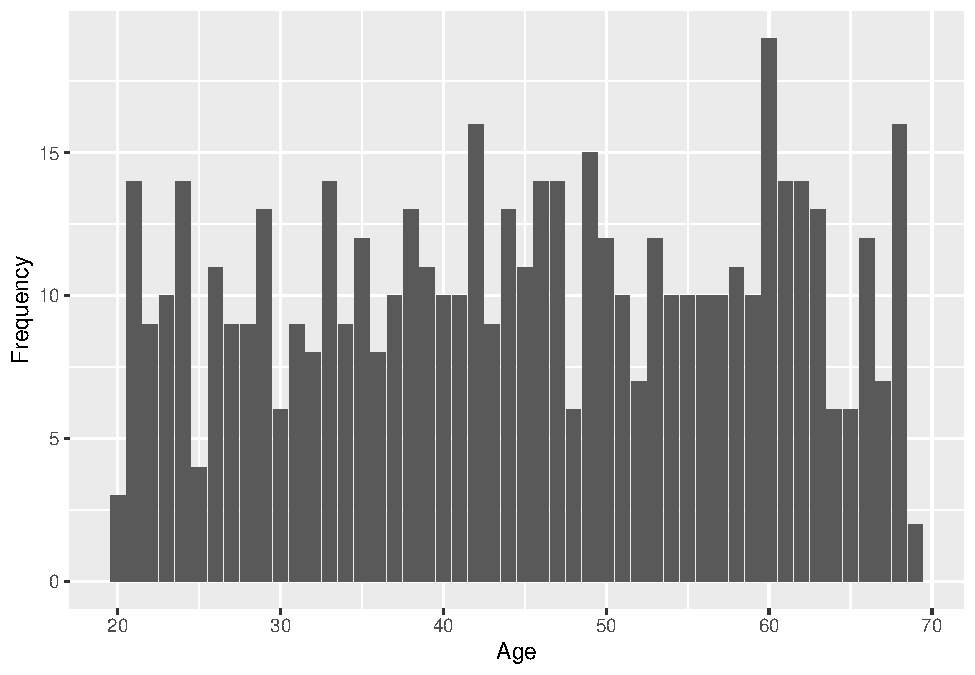
\includegraphics{report_files/figure-latex/age-dist-1.pdf}
\caption{\label{fig:age-dist}Distribution of age}
\end{figure}

Predictor \texttt{ethnicity} had 5 categories, with \texttt{non-hispanic\_white} being the most prevalent category with 220 cases (42\% of total), all the while \texttt{other} was the most infrequent category with 25 cases (5\%). A total of 525 cases contained \texttt{ethnicity} data, once again suggesting no presence of missing data values within this variable.

Predictor \texttt{education} was similar to \texttt{ethnicity}, having 5 categories. That said, the frequencies of said categories seemed to be less out of proportion, with \texttt{some\_college} being the most frequent category with 155 (30\%) cases. Whilst the data was retrieved from respondents of ages 20 and higher, no missing data values were observed within the variable. This could be further justified by the fact that the minimum \texttt{age} within the used dataset was 20, therefore foregoing possible issues with younger participants being unable to provide data for this specific variable.

The predictor variable \texttt{marital} contained 6 categories. It should be noted that the category value \texttt{married} exceeded the average frequency of other categories (that being 49.2) by a large margin, as can be seen in Figure \ref{fig:marital-dist-1}. Specifically, 279 cases (53\%) were \texttt{married}, with the other 5 categories making up the remaining 47\% of the cases. \texttt{never\_married} was the most frequent among those other 5 categories with 102 (19\%) cases, whilst \texttt{separated} was the most infrequent category with only 14 (3\%) cases. Furthermore, the meaning of \texttt{never\_married} and \texttt{living\_with\_partners} was ambiguous in the sense that a person specifically living with their (non-married) partner could fall into both these categories.

\begin{figure}
\centering
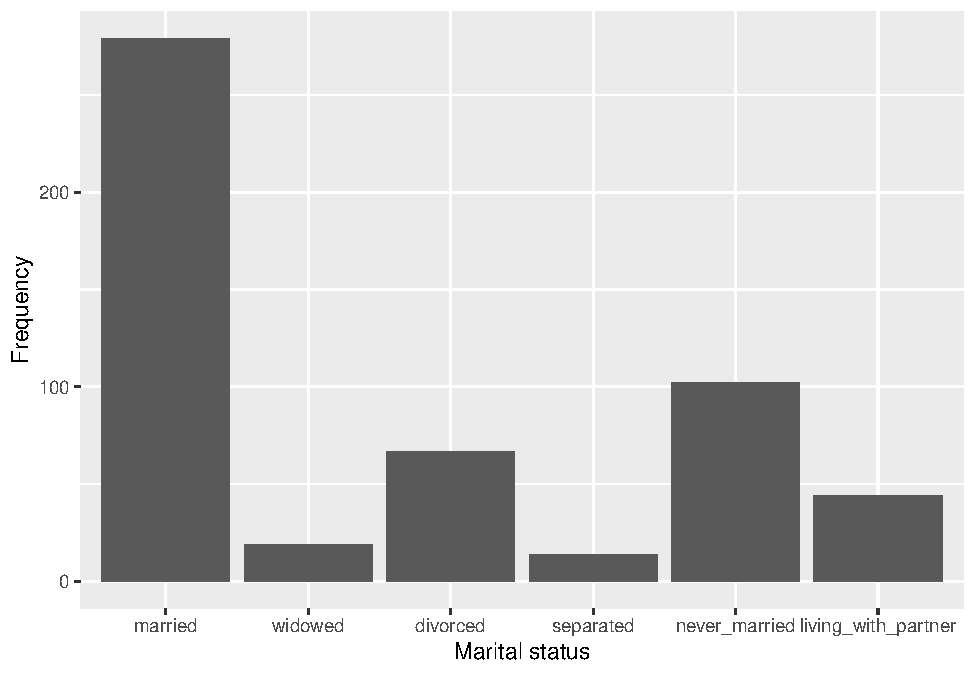
\includegraphics{report_files/figure-latex/marital-dist-1-1.pdf}
\caption{\label{fig:marital-dist-1}Distribution of marital status categories}
\end{figure}

Predictor \texttt{income} was an ordinal variable formed by 12 levels, ranging from income values 0 to 100000+. This data, like \texttt{age}, was topcoded at the value 100000. This also explained the highest income category - that being 100000+ - having 76 cases (9\%), as can be seen in Figure \ref{fig:income-dist}. If the latter case is ignored, the most frequent category was instead \texttt{25000:34999}, which coincidentally was the mid-range category of income data. 525 cases contained only observed \texttt{income} data, therefore the variable did not contain missing data values.

\begin{figure}
\centering
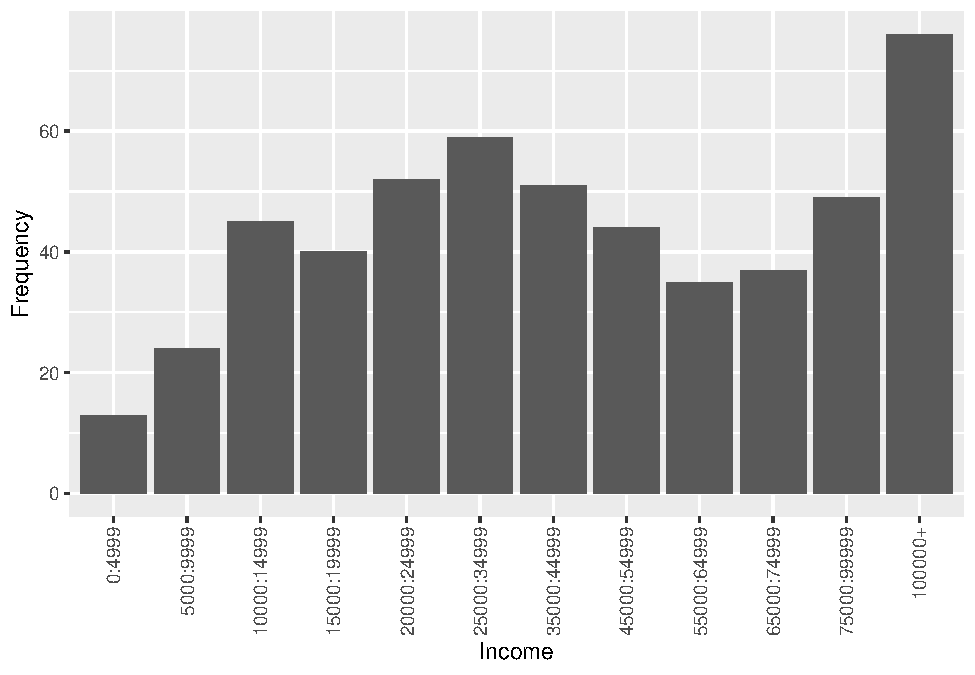
\includegraphics{report_files/figure-latex/income-dist-1.pdf}
\caption{\label{fig:income-dist}Distribution of income}
\end{figure}

The multiple levels of depression all had ranging scores between 0 and 3, with increments of 1 specifically. A higher score indicated an agreement with the signs of depression described in the survey. Only \texttt{dep1} and \texttt{dep7} had complete data data, whilst the other levels had varying amounts of missing data. Missing data could possibly be caused by the respondents being reluctant to answers these questions. It was also observed that \texttt{dep2}, \texttt{dep3}, \texttt{dep5}, \texttt{dep6} had the same amount of missing data values, hence it was possible that they had a shared cause of missing data. Lastly, \texttt{dep9} only had 18 cases of scores above 0, whilst also having the lowest mean value out of all depression levels. \texttt{dep9} described the presence of suicidal thoughts, hence it made sense that this was the lowest average score out of all levels. On the contrary, \texttt{dep4} (feeling tired) had the highest average score. Overall, the score distribution were heavily skewed towards the 0 values.

\hypertarget{outliers}{%
\subsection{Outliers}\label{outliers}}

For the only continuous predictor \texttt{age}, a boxplot was utilised to find potential outliers . Figure \ref{fig:age-outliers} shows the distribution of \texttt{age} in said boxplot, revealing no possible outliers. This was to be expected, since \texttt{age} was uniformly distributed as was mentioned in Section \ref{desc-stats}.

\begin{figure}
\centering
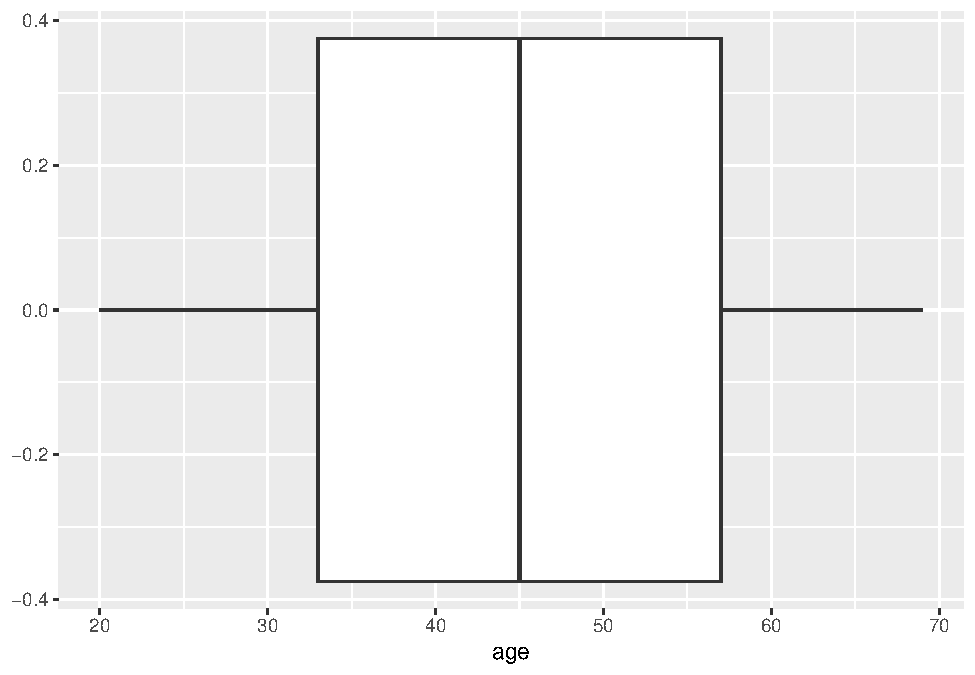
\includegraphics{report_files/figure-latex/age-outliers-1.pdf}
\caption{\label{fig:age-outliers}Boxplot of age}
\end{figure}

Looking at the distributions of the various categorical variables, the \texttt{marital} showed the aforementioned imbalance in frequency distribution, with the category \texttt{married} being overly dominant within the data. It was considered combining the other \texttt{marital} categories into one, as their infrequency could allude to being possible outliers. Table \ref{tab:cont-marital} shows the interrelations between the \texttt{martial} variable and the outcome \texttt{drink\_regularly}. From this, it was concluded that combining the remaining 5 categories - that being \texttt{widowed}, \texttt{divorced}, \texttt{separated}, \texttt{never\_married} and \texttt{living\_with\_partner} - was not feasible, since these relations seemed to differ per category. For example, \texttt{widowed} had more ``no'' cases compared to ``yes'', whilst the relation was reversed for \texttt{separated}.

\begin{table}[!h]

\caption{\label{tab:cont-marital}Contingency table of marital status vs. drinking regularly}
\centering
\begin{tabular}[t]{lrr}
\toprule
  & no & yes\\
\midrule
\cellcolor{gray!6}{married} & \cellcolor{gray!6}{81} & \cellcolor{gray!6}{175}\\
widowed & 11 & 8\\
\cellcolor{gray!6}{divorced} & \cellcolor{gray!6}{14} & \cellcolor{gray!6}{48}\\
separated & 4 & 8\\
\cellcolor{gray!6}{never\_married} & \cellcolor{gray!6}{23} & \cellcolor{gray!6}{45}\\
\addlinespace
living\_with\_partner & 6 & 23\\
\bottomrule
\end{tabular}
\end{table}

\hypertarget{correlations}{%
\subsection{Correlations}\label{correlations}}

\begin{figure}
\centering
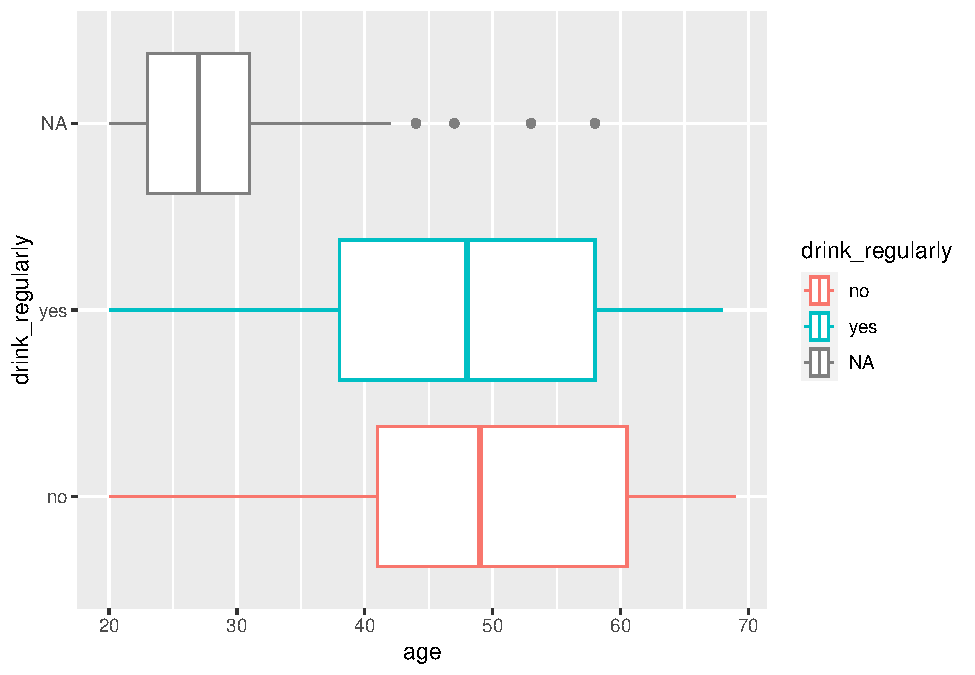
\includegraphics{report_files/figure-latex/box-age-1.pdf}
\caption{\label{fig:box-age}Correlations of age vs.~drink regularly}
\end{figure}

Figure \ref{fig:box-age} shows the distributions of \texttt{age} over the outcome variable \texttt{drink\_regularly} in a boxplot. Not considering the NA values, \texttt{age} did not seem to be strongly correlated with \texttt{drink\_regularly}, with ``no'' cases having only slightly higher ages than its counterpart. It should however be noted that the NA values of \texttt{drink\_regularly} were primarily present in younger participants, therefore possibly attenuating the correlation effect between these two variables. For example, a large amount of missing values belonging to ``yes'' could shift the distribution of these cases towards lower \texttt{age} values, hence increasing the difference in distributions for each \texttt{drink\_regularly} outcome.

Contingency tables and frequency distribution plots (including NA values) were used to observe the correlation between the categorical predictors and the outcome variable. From these, it was observed that \texttt{sex} seemed to be highly correlated with \texttt{drink\_regularly}; 172 cases of \texttt{male} drank regularly, whilst only 39 didn't. Compared to the 135 cases of \texttt{female} of ``yes'' and 100 cases of ``no'', this ratio seemed to differ greatly per \texttt{sex} category. The missingness of \texttt{drink\_regularly} was evenly distributed across both \texttt{male} and \texttt{female} cases.

\begin{figure}
\centering
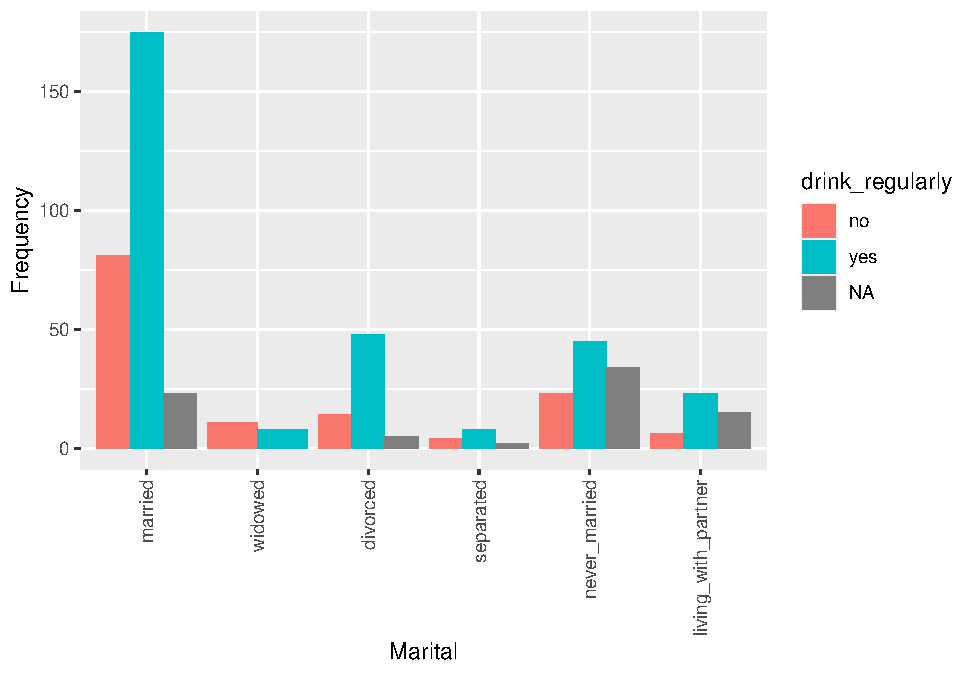
\includegraphics{report_files/figure-latex/cor-marital-1.pdf}
\caption{\label{fig:cor-marital}Correlations of marital vs.~drink regularly}
\end{figure}

Likewise, \texttt{marital} showed a similarly strong correlation effect. The category \texttt{divorced} had a significantly higher ratio of respondents who drank regularly, compared to cases of \texttt{widowed}, where respondents were more likely to not drink regularly as can be seen in Figure \ref{fig:cor-marital}. It was also noted that the missing data of \texttt{drink\_regularly} was not evenly distributed across the \texttt{marital} categories. Rather, the missingness was more prevalent in the \texttt{never\_married} and \texttt{living\_with\_partner} cases. This possibly ties back into the fact that more data was missing amongst younger respondents, which can be direcly seen in Figure \ref{fig:age-marital} where \texttt{never\_married} and \texttt{living\_with\_partner} have more cases of a younger age as well.

\begin{figure}
\centering
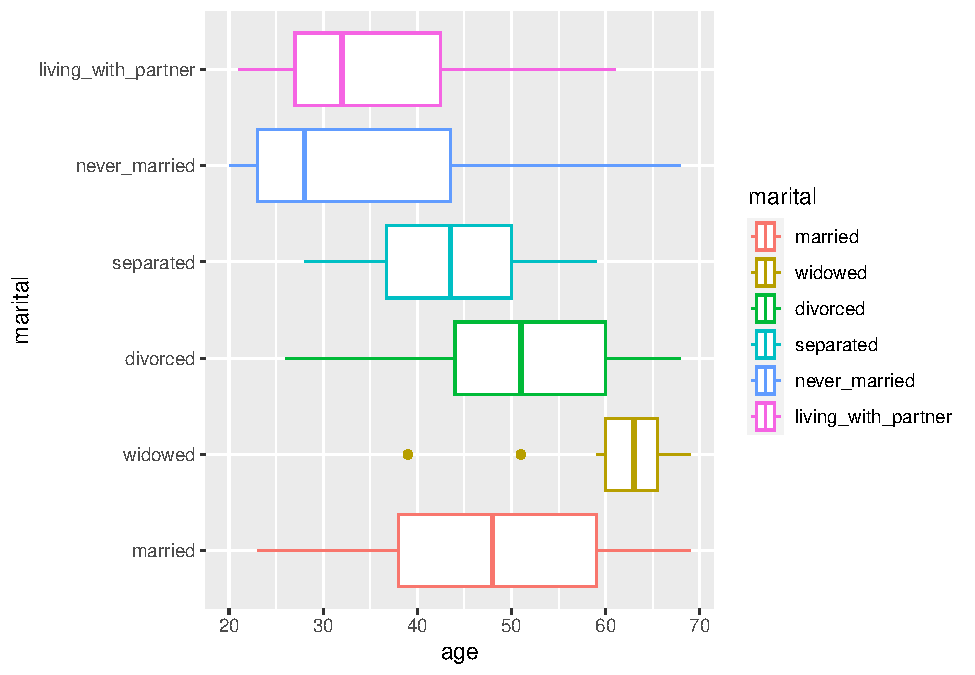
\includegraphics{report_files/figure-latex/age-marital-1.pdf}
\caption{\label{fig:age-marital}Age distributions over marital statuses}
\end{figure}

\texttt{Ethnicity} showed a weaker correlation effect with the outcome variable. Only \texttt{non-hispanic\_black} and \texttt{other} showed different frequency distributions compared to the other categories. Missing data of \texttt{drink\_regularly} was present in all categories of \texttt{ethnicity}, though \texttt{other\_hispanic} and \texttt{other} had close to none compared to the remaining categories.
The variable \texttt{education} was considered to have the weakest correlation with \texttt{drink\_regularly}, having similar success ratios across all categories all the while missing data of \texttt{drink\_regularly} was also evenly spread.

\texttt{income} was considered to be correlated with the outcome variable. Performing a similar analysis, it was observed that respondents with an income up until 24999 were less likely to drink regularly than cases with a higher income. Akin to \texttt{education}, missing data of \texttt{drink\_regularly} seemed to be evenly spread across the \texttt{income} values.

Finally, all levels of depression showed an effect of correlation with \texttt{drink\_regularly}, where higher scores tended to decrease the ratio of ``yes'' to ``no'' cases, that is to say that respondents were less likely to drink regularly if signs of depression were present.

\hypertarget{missing-data-problem}{%
\section{Missing data problem}\label{missing-data-problem}}

\hypertarget{missing-data-and-response-patterns}{%
\subsection{Missing data and response patterns}\label{missing-data-and-response-patterns}}

Firstly, the overall distribution of missingness within the dataset was investigated.

\begin{figure}
\centering
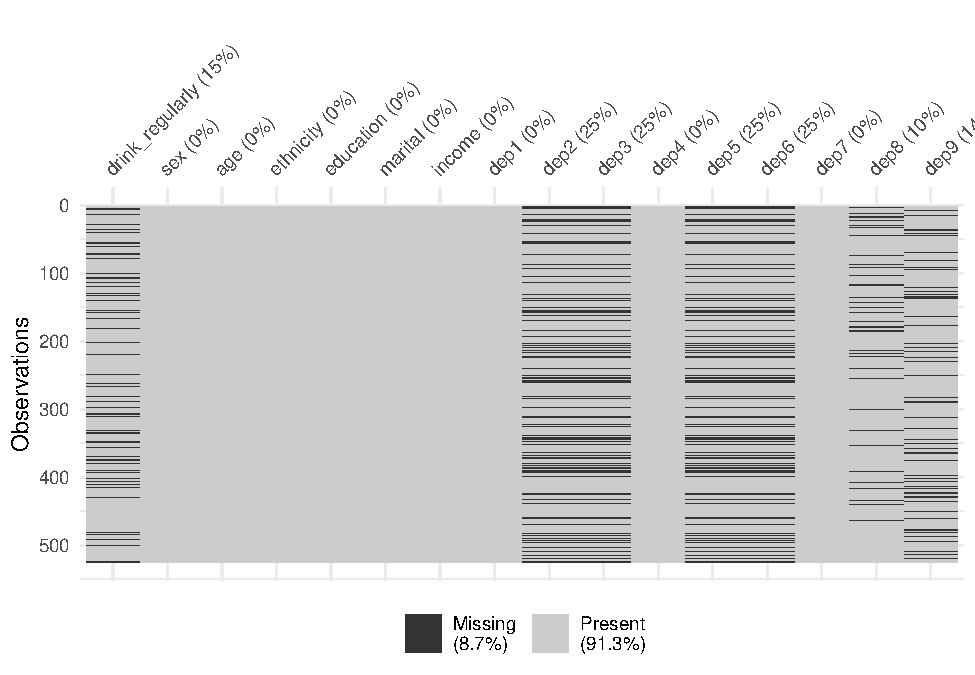
\includegraphics{report_files/figure-latex/mis-percentage-1.pdf}
\caption{\label{fig:mis-percentage}Distribution of missing data in each variable}
\end{figure}

As can be seen on Figure \ref{fig:mis-percentage}, 8.2\% of the data was missing. The missing values occurred in the outcome variable \texttt{drink\_regularly} and in the responses to questions \texttt{dep2}, \texttt{dep3}, \texttt{dep5}, \texttt{dep6}, \texttt{dep8} and \texttt{dep9} that created the depression score variable. 15\% of responses were missing for the predictor variable. 25\% of the responses were missing for the individual depression questions 2, 3, 5 and 6, whilst 10\% were missing for question 8. Finally, 14\% of data was missing for question 9.

\begin{figure}
\centering
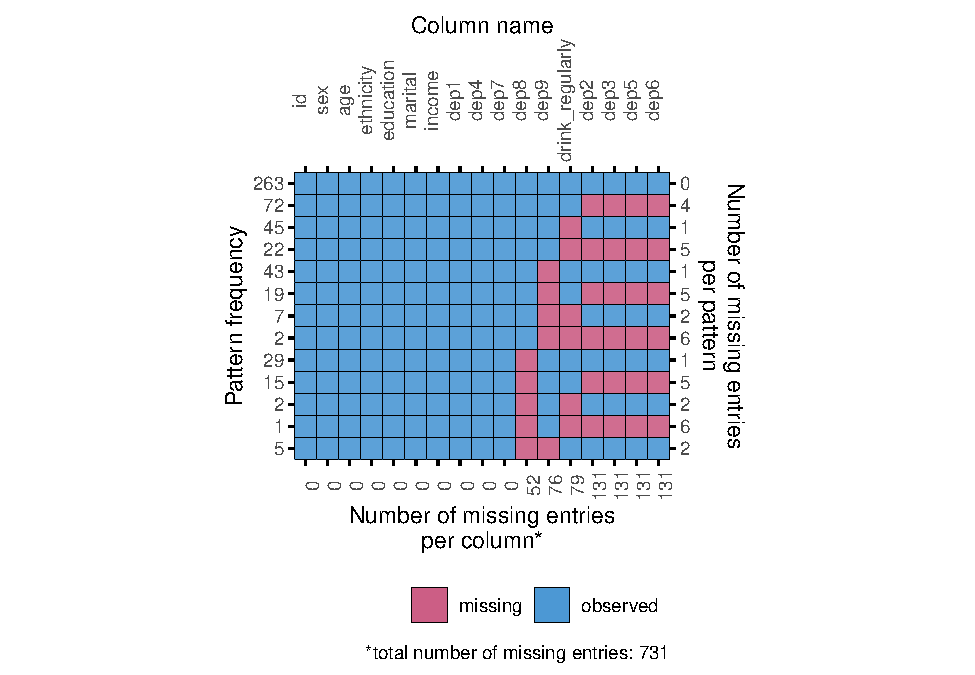
\includegraphics{report_files/figure-latex/res-pattern-1.pdf}
\caption{\label{fig:res-pattern}Response patterns and their frequency}
\end{figure}

The missing data patterns were further investigated by looking at the response patterns. Figure \ref{fig:res-pattern} reveals that there were 13 distinct response patterns in the dataset, with the missingness \emph{not} being monotone. The most frequent pattern was no missing entries, with 263 cases. It is important to note that the depression questions 2, 3, 5 and 6 were always either all present or all missing. It is very probable that the reason for the item non-response regarding these depression levels was the same, since there were no cases with partial missingness in these 4 variables.

Based on the missingness pattern of the depression items, 41\% of the overall depression score included at least one missing value.

\hypertarget{MDM}{%
\subsection{Missing data mechanism}\label{MDM}}

Missing completely at random (MCAR) missingness mechanism is often an important assumption for statistical analysis, including this one. To gain some inside whether the data was MCAR or not, we deployed a variety of tests. If missing values of a variable was MCAR, said variable should not have a significant dependency with other (observed) variables.

Firstly, Little MCAR test was performed to verify if the missing data was MCAR at a global level, thus for all of the instances of missingess. The test was significant (\(\chi^2 (164) = 465.18, p < 0.01\)), therefore the data was assumed to \emph{not} be MCAR.

Since the data being MCAR can be questioned following the Little's test, a t-test was performed for all missing values vectors and numerical variables to check which variables were the likely culprit. The test compared the observed means of a given numerical variable within the group of individuals that had an observed value and the group with a missing value for another variable. Effectively testing if there is a significant difference in the continuous variable in the group that answered another question and the group that did not. Since the null hypothesis suggests no difference in means across the groups, a single significant value for a missingness of a given variable suggests that the missing values in that variable depend on the observed values of another variable. Therefore, it is likely that the missing values are not MCAR. Due to the identical pattern of responses in \texttt{dep2}, \texttt{dep3}, \texttt{dep5} and \texttt{dep6} it was sufficient to only test once for the dependency of their missing values. By the design of the test, it was impossible to test the dependency of missing values and observed values within the same variable, thus these values were missing from the table.

Assuming an alpha of 0.05, it was observed that missing values of \texttt{drink\_regularly} were dependent on \texttt{age}, \texttt{dep2} and \texttt{dep9}. Similarly, \texttt{dep2}, \texttt{dep3}, \texttt{dep5} and \texttt{dep6} seemed to be dependent on \texttt{age} and the remaining depression questions. For missingness in \texttt{dep8} and \texttt{dep9}, there were no significant differences across groups in any of the numerical variables. These tests suggested that at least \texttt{drink\_regularly}, \texttt{dep2}, \texttt{dep3}, \texttt{dep5} and \texttt{dep6} were not MCAR, thus MAR was assumed for them. In Table \ref{tab:is-mis-vectors} the exact t-statistic and the p-value are reported.

\begin{table}[!h]

\caption{\label{tab:is-mis-vectors}Dependency t-test: mean comparison in numerical variables across missing values and observed values in the other variables}
\centering
\resizebox{\linewidth}{!}{
\begin{tabular}[t]{lllll}
\toprule
numerical variable & missing drink\_regularly & missing dep2/3/5/6 & missing dep8 & missing dep9\\
\midrule
\cellcolor{gray!6}{age} & \cellcolor{gray!6}{t = 19.3, pVal = 3.1e-45} & \cellcolor{gray!6}{t = 1.38, pVal = 0.17} & \cellcolor{gray!6}{t = -1.16, pVal = 0.249} & \cellcolor{gray!6}{t = -0.884, pVal = 0.379}\\
dep1 & t = 1.39, pVal = 0.167 & t = -6.72, pVal = 2.88e-10 & t = 0.464, pVal = 0.644 & t = -0.444, pVal = 0.658\\
\cellcolor{gray!6}{dep2} & \cellcolor{gray!6}{t = 3.63, pVal = 0.000405} & \cellcolor{gray!6}{-} & \cellcolor{gray!6}{t = 0.332, pVal = 0.742} & \cellcolor{gray!6}{t = 1.22, pVal = 0.224}\\
dep3 & t = 0.797, pVal = 0.428 & - & t = -0.137, pVal = 0.892 & t = 0.0545, pVal = 0.957\\
\cellcolor{gray!6}{dep4} & \cellcolor{gray!6}{t = -0.541, pVal = 0.59} & \cellcolor{gray!6}{t = -7.8, pVal = 6.11e-13} & \cellcolor{gray!6}{t = -0.68, pVal = 0.499} & \cellcolor{gray!6}{t = -1.28, pVal = 0.202}\\
\addlinespace
dep5 & t = 2.01, pVal = 0.0466 & - & t = -0.605, pVal = 0.549 & t = -0.731, pVal = 0.467\\
\cellcolor{gray!6}{dep6} & \cellcolor{gray!6}{t = 0.822, pVal = 0.414} & \cellcolor{gray!6}{-} & \cellcolor{gray!6}{t = 2.3, pVal = 0.0242} & \cellcolor{gray!6}{t = 0.00637, pVal = 0.995}\\
dep7 & t = -0.382, pVal = 0.703 & t = -8.19, pVal = 1.24e-13 & t = -0.239, pVal = 0.812 & t = -0.0635, pVal = 0.949\\
\cellcolor{gray!6}{dep8} & \cellcolor{gray!6}{t = -0.32, pVal = 0.75} & \cellcolor{gray!6}{t = -4.26, pVal = 3.86e-05} & \cellcolor{gray!6}{-} & \cellcolor{gray!6}{t = 0.595, pVal = 0.553}\\
dep9 & t = 2.48, pVal = 0.0135 & t = -2.64, pVal = 0.00947 & t = -0.295, pVal = 0.769 & -\\
\bottomrule
\end{tabular}}
\end{table}

\begin{table}[!h]

\caption{\label{tab:chi-squared-test}Independency Chi-squared test}
\centering
\resizebox{\linewidth}{!}{
\begin{tabular}[t]{lllll}
\toprule
categorical variable & missing drink\_regularly & missing dep2/3/5/6 & missing dep8 & missing dep9\\
\midrule
\cellcolor{gray!6}{drink\_regularly} & \cellcolor{gray!6}{-} & \cellcolor{gray!6}{X\textasciicircum{}2 = 4.2, pVal = 0.0404} & \cellcolor{gray!6}{X\textasciicircum{}2 = 1.52, pVal = 0.218} & \cellcolor{gray!6}{X\textasciicircum{}2 = 0.464, pVal = 0.496}\\
sex & X\textasciicircum{}2 = 1.09, pVal = 0.296 & X\textasciicircum{}2 = 5.04, pVal = 0.0248 & X\textasciicircum{}2 = 0.469, pVal = 0.494 & X\textasciicircum{}2 = 0.317, pVal = 0.573\\
\cellcolor{gray!6}{ethnicity} & \cellcolor{gray!6}{X\textasciicircum{}2 = 5.49, pVal = 0.241} & \cellcolor{gray!6}{X\textasciicircum{}2 = 1.64, pVal = 0.802} & \cellcolor{gray!6}{X\textasciicircum{}2 = 7.74, pVal = 0.102} & \cellcolor{gray!6}{X\textasciicircum{}2 = 5.8, pVal = 0.215}\\
education & X\textasciicircum{}2 = 2.7, pVal = 0.609 & X\textasciicircum{}2 = 5.72, pVal = 0.221 & X\textasciicircum{}2 = 1.63, pVal = 0.803 & X\textasciicircum{}2 = 5.13, pVal = 0.275\\
\cellcolor{gray!6}{marital} & \cellcolor{gray!6}{X\textasciicircum{}2 = 55.7, pVal = 9.58e-11} & \cellcolor{gray!6}{X\textasciicircum{}2 = 22.2, pVal = 0.000477} & \cellcolor{gray!6}{X\textasciicircum{}2 = 5.08, pVal = 0.407} & \cellcolor{gray!6}{X\textasciicircum{}2 = 3.97, pVal = 0.553}\\
\addlinespace
income & X\textasciicircum{}2 = 2.94, pVal = 0.991 & X\textasciicircum{}2 = 8.84, pVal = 0.636 & X\textasciicircum{}2 = 9.4, pVal = 0.585 & X\textasciicircum{}2 = 17.3, pVal = 0.0995\\
\bottomrule
\end{tabular}}
\end{table}

Since the t-test was not appropriate for categorical variables, we performed the Chi-squared test for said variables. The null hypothesis of the tests entailed no significant relationships between the categorical variables. The test compared observed frequencies to expected frequencies, if there was no relationship between the variables.

The outcomes of the test are presented in Table \ref{tab:chi-squared-test}. However, only \texttt{martial} with missingness of \texttt{drink\_regularly} and \texttt{marital} with missingness of \texttt{dep2}, \texttt{dep3}, \texttt{dep5} and \texttt{dep6} were significant. Thus, it further supported the non-MCAR behaviour of missing data in these items.

However, the Chi-squared test had an requirement that the smallest expected frequencies had to be higher than 5. This requirement was not met for some combinations of missing values and categorical variables. Specifically: missing \texttt{dep8/9} and \texttt{ethnicity}, \texttt{marital}, \texttt{income}; missing \texttt{dep2/3/5/6} and \texttt{marital}, \texttt{income}; missing \texttt{drink\_regularly} and \texttt{ethnicity}, \texttt{marital}, \texttt{income}. Since this assumption was not met for these combination, the p-values might not have been correctly estimated. Therefore, the Fischer test - which has the same hypothesis, but not the same assumption - was performed for these combinations.

\begin{table}[!h]

\caption{\label{tab:fisher-test}Fisher test}
\centering
\resizebox{\linewidth}{!}{
\begin{tabular}[t]{lllll}
\toprule
categorical variable & missing drink\_regularly & missing dep2/3/5/6 & missing dep8 & missing dep9\\
\midrule
\cellcolor{gray!6}{ethnicity} & \cellcolor{gray!6}{pVal = 0.235} & \cellcolor{gray!6}{-} & \cellcolor{gray!6}{pVal = 0.0817} & \cellcolor{gray!6}{pVal = 0.211}\\
marital & pVal = 1e-05 & pVal = 0.00074 & pVal = 0.403 & pVal = 0.446\\
\cellcolor{gray!6}{income} & \cellcolor{gray!6}{pVal = 0.988} & \cellcolor{gray!6}{pVal = 0.643} & \cellcolor{gray!6}{pVal = 0.56} & \cellcolor{gray!6}{pVal = 0.0597}\\
\bottomrule
\end{tabular}}
\end{table}

The outcomes of the Fisher test are presented in Table \ref{tab:fisher-test}. Like in the case of Chi-squared test, only \texttt{martial} with missingness of \texttt{drink\_regularly} and \texttt{marital} with missingness of \texttt{dep2}, \texttt{dep3}, \texttt{dep5} and \texttt{dep6} were significant. Therefore, it was concluded the dependence of missingness in these variables on multiple other observed variables and rejected MCAR in their case.

In all of the tests above, \texttt{dep8} and \texttt{dep9} did not seem to be dependent on any of the observed variables. Thus, perhaps MCAR could be assumed for these variables. However, since the depression scores will be collapsed into a single depression score (`dep') and other depression questions were MAR, the overall score was also assumed to be MAR.

\hypertarget{imputation}{%
\section{Imputation results}\label{imputation}}

\begin{verbatim}
##                   sex age ethnicity education marital household_size income
## sex                 0   1         1         1       1              1      1
## age                 1   0         1         1       1              1      1
## ethnicity           1   1         0         1       1              1      1
## education           1   1         1         0       1              1      1
## marital             1   1         1         1       0              1      1
## household_size      1   1         1         1       1              0      1
## income              1   1         1         1       1              1      0
## weight              1   1         1         1       1              1      1
## height              1   1         1         1       1              1      1
## bmi                 1   1         1         1       1              1      1
## pulse               1   1         1         1       1              1      1
## bp_sys1             1   1         1         1       1              1      1
## bp_dia1             1   1         1         1       1              1      1
## bp_sys2             1   1         1         1       1              1      1
## bp_dia2             1   1         1         1       1              1      1
## vig_work            1   1         1         1       1              1      1
## mod_work            1   1         1         1       1              1      1
## walk_cycle          1   1         1         1       1              1      1
## vig_rec             1   1         1         1       1              1      1
## mod_rec             1   1         1         1       1              1      1
## time_sed            1   1         1         1       1              1      1
## n_sex_year          1   1         1         1       1              1      1
## n_unsafe_sex_year   1   1         1         1       1              1      1
## drink_regularly     1   1         1         1       1              1      1
## days_drinking       1   1         1         1       1              1      1
## dep1                1   1         1         1       1              1      1
## dep2                1   1         1         1       1              1      1
## dep3                1   1         1         1       1              1      1
## dep4                1   1         1         1       1              1      1
## dep5                1   1         1         1       1              1      1
## dep6                1   1         1         1       1              1      1
## dep7                1   1         1         1       1              1      1
## dep8                1   1         1         1       1              1      1
## dep9                1   1         1         1       1              1      1
##                   weight height bmi pulse bp_sys1 bp_dia1 bp_sys2 bp_dia2
## sex                    1      1   1     1       1       1       1       1
## age                    1      1   1     1       1       1       1       1
## ethnicity              1      1   1     1       1       1       1       1
## education              1      1   1     1       1       1       1       1
## marital                1      1   1     1       1       1       1       1
## household_size         1      1   1     1       1       1       1       1
## income                 1      1   1     1       1       1       1       1
## weight                 0      1   1     1       1       1       1       1
## height                 1      0   1     1       1       1       1       1
## bmi                    1      1   0     1       1       1       1       1
## pulse                  1      1   1     0       1       1       1       1
## bp_sys1                1      1   1     1       0       1       1       1
## bp_dia1                1      1   1     1       1       0       1       1
## bp_sys2                1      1   1     1       1       1       0       1
## bp_dia2                1      1   1     1       1       1       1       0
## vig_work               1      1   1     1       1       1       1       1
## mod_work               1      1   1     1       1       1       1       1
## walk_cycle             1      1   1     1       1       1       1       1
## vig_rec                1      1   1     1       1       1       1       1
## mod_rec                1      1   1     1       1       1       1       1
## time_sed               1      1   1     1       1       1       1       1
## n_sex_year             1      1   1     1       1       1       1       1
## n_unsafe_sex_year      1      1   1     1       1       1       1       1
## drink_regularly        1      1   1     1       1       1       1       1
## days_drinking          1      1   1     1       1       1       1       1
## dep1                   1      1   1     1       1       1       1       1
## dep2                   1      1   1     1       1       1       1       1
## dep3                   1      1   1     1       1       1       1       1
## dep4                   1      1   1     1       1       1       1       1
## dep5                   1      1   1     1       1       1       1       1
## dep6                   1      1   1     1       1       1       1       1
## dep7                   1      1   1     1       1       1       1       1
## dep8                   1      1   1     1       1       1       1       1
## dep9                   1      1   1     1       1       1       1       1
##                   vig_work mod_work walk_cycle vig_rec mod_rec time_sed
## sex                      1        1          1       1       1        1
## age                      1        1          1       1       1        1
## ethnicity                1        1          1       1       1        1
## education                1        1          1       1       1        1
## marital                  1        1          1       1       1        1
## household_size           1        1          1       1       1        1
## income                   1        1          1       1       1        1
## weight                   1        1          1       1       1        1
## height                   1        1          1       1       1        1
## bmi                      1        1          1       1       1        1
## pulse                    1        1          1       1       1        1
## bp_sys1                  1        1          1       1       1        1
## bp_dia1                  1        1          1       1       1        1
## bp_sys2                  1        1          1       1       1        1
## bp_dia2                  1        1          1       1       1        1
## vig_work                 0        1          1       1       1        1
## mod_work                 1        0          1       1       1        1
## walk_cycle               1        1          0       1       1        1
## vig_rec                  1        1          1       0       1        1
## mod_rec                  1        1          1       1       0        1
## time_sed                 1        1          1       1       1        0
## n_sex_year               1        1          1       1       1        1
## n_unsafe_sex_year        1        1          1       1       1        1
## drink_regularly          1        1          1       1       1        1
## days_drinking            1        1          1       1       1        1
## dep1                     1        1          1       1       1        1
## dep2                     1        1          1       1       1        1
## dep3                     1        1          1       1       1        1
## dep4                     1        1          1       1       1        1
## dep5                     1        1          1       1       1        1
## dep6                     1        1          1       1       1        1
## dep7                     1        1          1       1       1        1
## dep8                     1        1          1       1       1        1
## dep9                     1        1          1       1       1        1
##                   n_sex_year n_unsafe_sex_year drink_regularly days_drinking
## sex                        1                 1               1             1
## age                        1                 1               1             1
## ethnicity                  1                 1               1             1
## education                  1                 1               1             1
## marital                    1                 1               1             1
## household_size             1                 1               1             1
## income                     1                 1               1             1
## weight                     1                 1               1             1
## height                     1                 1               1             1
## bmi                        1                 1               1             1
## pulse                      1                 1               1             1
## bp_sys1                    1                 1               1             1
## bp_dia1                    1                 1               1             1
## bp_sys2                    1                 1               1             1
## bp_dia2                    1                 1               1             1
## vig_work                   1                 1               1             1
## mod_work                   1                 1               1             1
## walk_cycle                 1                 1               1             1
## vig_rec                    1                 1               1             1
## mod_rec                    1                 1               1             1
## time_sed                   1                 1               1             1
## n_sex_year                 0                 1               1             1
## n_unsafe_sex_year          1                 0               1             1
## drink_regularly            1                 1               0             1
## days_drinking              1                 1               1             0
## dep1                       1                 1               1             1
## dep2                       1                 1               1             1
## dep3                       1                 1               1             1
## dep4                       1                 1               1             1
## dep5                       1                 1               1             1
## dep6                       1                 1               1             1
## dep7                       1                 1               1             1
## dep8                       1                 1               1             1
## dep9                       1                 1               1             1
##                   dep1 dep2 dep3 dep4 dep5 dep6 dep7 dep8 dep9
## sex                  1    1    1    1    1    1    1    1    1
## age                  1    1    1    1    1    1    1    1    1
## ethnicity            1    1    1    1    1    1    1    1    1
## education            1    1    1    1    1    1    1    1    1
## marital              1    1    1    1    1    1    1    1    1
## household_size       1    1    1    1    1    1    1    1    1
## income               1    1    1    1    1    1    1    1    1
## weight               1    1    1    1    1    1    1    1    1
## height               1    1    1    1    1    1    1    1    1
## bmi                  1    1    1    1    1    1    1    1    1
## pulse                1    1    1    1    1    1    1    1    1
## bp_sys1              1    1    1    1    1    1    1    1    1
## bp_dia1              1    1    1    1    1    1    1    1    1
## bp_sys2              1    1    1    1    1    1    1    1    1
## bp_dia2              1    1    1    1    1    1    1    1    1
## vig_work             1    1    1    1    1    1    1    1    1
## mod_work             1    1    1    1    1    1    1    1    1
## walk_cycle           1    1    1    1    1    1    1    1    1
## vig_rec              1    1    1    1    1    1    1    1    1
## mod_rec              1    1    1    1    1    1    1    1    1
## time_sed             1    1    1    1    1    1    1    1    1
## n_sex_year           1    1    1    1    1    1    1    1    1
## n_unsafe_sex_year    1    1    1    1    1    1    1    1    1
## drink_regularly      1    1    1    1    1    1    1    1    1
## days_drinking        1    1    1    1    1    1    1    1    1
## dep1                 0    1    1    1    1    1    1    1    1
## dep2                 1    0    1    1    1    1    1    1    1
## dep3                 1    1    0    1    1    1    1    1    1
## dep4                 1    1    1    0    1    1    1    1    1
## dep5                 1    1    1    1    0    1    1    1    1
## dep6                 1    1    1    1    1    0    1    1    1
## dep7                 1    1    1    1    1    1    0    1    1
## dep8                 1    1    1    1    1    1    1    0    1
## dep9                 1    1    1    1    1    1    1    1    0
\end{verbatim}

Four imputed datasets were created for the analysis models. The imputed values of interest were \texttt{drink\_regularly}, \texttt{dep2}, \texttt{dep3}, \texttt{dep5}, \texttt{dep6}, \texttt{dep8}, \texttt{dep9}.

\hypertarget{lw}{%
\subsection{List-wise deletion}\label{lw}}

The data before applying list-wise deletion had 525 cases. After performing the deletion-based treatment, the resulting dataset had 263 cases left. The ratio of ``yes'' to ``no'' cases in the outcome variable \texttt{drink\_regularly} changed from 2.21 to 1.86, hence decreasing by -15.84\%.

Table \ref{tab:dep-means-lw} shows the means of the multiple depression levels in the original data set and the resulting dataset from list-wise deletion. It was observed that the mean values of \texttt{dep8} and \texttt{dep9} decreased by half in the resulting dataset, suggesting that this missing data treatment deleted cases with higher \texttt{dep8} and \texttt{dep9} values due to missing values in either \texttt{drink\_regularly} or the depression levels. The mean values of the remaining levels stayed roughly the same, showing no significant increase or decrease.

\begin{table}[!h]

\caption{\label{tab:dep-means-lw}Depression means for list-wise deletion}
\centering
\begin{tabular}[t]{lrrrrrr}
\toprule
data & dep2 & dep3 & dep5 & dep6 & dep8 & dep9\\
\midrule
\cellcolor{gray!6}{original} & \cellcolor{gray!6}{0.282} & \cellcolor{gray!6}{0.533} & \cellcolor{gray!6}{0.310} & \cellcolor{gray!6}{0.201} & \cellcolor{gray!6}{0.203} & \cellcolor{gray!6}{0.067}\\
result & 0.323 & 0.544 & 0.304 & 0.217 & 0.118 & 0.030\\
\bottomrule
\end{tabular}
\end{table}

Table \ref{tab:dep-vars-lw} shows the change of variance across the multiple depression levels. Similar to the affect on mean values, variances of depression only showed significant changes in \texttt{dep8} and \texttt{dep9}, furthermore suggesting that missing data was present in other variables for particular \texttt{dep8} and \texttt{dep9} values respectively. The other depression levels showed only small increases or decrease in variance, which is due to the sampling variability as a consequence of list-wise deletion. Although \texttt{dep8} and \texttt{dep9} were assumed to be MCAR in Section \ref{MDM}, these did in fact show the most substantial changes in their distribution.

\begin{table}[!h]

\caption{\label{tab:dep-vars-lw}Depression variance for list-wise deletion}
\centering
\begin{tabular}[t]{lrrrrrr}
\toprule
data & dep2 & dep3 & dep5 & dep6 & dep8 & dep9\\
\midrule
\cellcolor{gray!6}{original} & \cellcolor{gray!6}{0.34} & \cellcolor{gray!6}{0.733} & \cellcolor{gray!6}{0.494} & \cellcolor{gray!6}{0.318} & \cellcolor{gray!6}{0.344} & \cellcolor{gray!6}{0.138}\\
result & 0.38 & 0.677 & 0.487 & 0.331 & 0.196 & 0.053\\
\bottomrule
\end{tabular}
\end{table}

TODO: explain the above, why?!

Lastly, the depression values were still discrete - the values ranged from 0 to 3. This was expected, since this missing data treatment didn't change / impute the values of the dataset.

\hypertarget{mean-imputation}{%
\subsection{Mean imputation}\label{mean-imputation}}

Mode imputation was applied to the missing values in \texttt{drink\_regularly}. As mentioned in Section \ref{data-proc}, ``yes'' was the most occuring case in the outcome variable, therefore missing values were replaced by ``yes''. This resulted in the ratio of ``yes'' to ``no'' cases changing from 2.21 to 2.78, increasing by 25.79\%. It is worthy to note that this is a 41.63\% total increase compared to the ratio of list-wise deletion mentioned in Section \ref{lw}.
As for the depression levels, mean imputation did not change the mean values. The overall variance of the depression levels decreased, which is an expected result of mean imputation - imputing missing data with the same value attenuates the variance of the variable.

\hypertarget{stochastic-regression}{%
\subsection{Stochastic regression}\label{stochastic-regression}}

The 3rd imputation method utilised a single stochastic regression model to treat the missing. The ratio of ``yes'' to ``no'' cases in the outcome variable \texttt{drink\_regularly} showed minimal change when observing the imputed data, with the original and imputed data having a ratio of 2.21 and 2.22 respectively.\\
Due to the nature of the stochastic regression model, the range of 0 to 3 with increments of 1 no longer held. To illustrate, \texttt{dep2} had a minimum value of -1.2 and a maximum value of 3.17, with values other than 0, 1, 2 or 3 existing within the variable. This also caused the variance of the assumed MAR depression levels to increase, as can be seen in Table \ref{tab:dep-vars-si}. The assumed MCAR depression variables - namely \texttt{dep8} and \texttt{dep9} - showed non-substantial increases in their variance. The proportional change in the mean values was also only present in \texttt{dep2}, \texttt{dep3}, \texttt{dep5} and \texttt{dep6}, whilst the assumed MCAR levels once again showed minimal change, as shown in Table \ref{tab:dep-means-si}.

\begin{table}[!h]

\caption{\label{tab:dep-means-si}Depression means for stochastic regression}
\centering
\begin{tabular}[t]{lrrrrrr}
\toprule
data & dep2 & dep3 & dep5 & dep6 & dep8 & dep9\\
\midrule
\cellcolor{gray!6}{original} & \cellcolor{gray!6}{0.282} & \cellcolor{gray!6}{0.533} & \cellcolor{gray!6}{0.310} & \cellcolor{gray!6}{0.201} & \cellcolor{gray!6}{0.203} & \cellcolor{gray!6}{0.067}\\
result & 0.415 & 0.701 & 0.395 & 0.359 & 0.202 & 0.066\\
\bottomrule
\end{tabular}
\end{table}

\begin{table}[!h]

\caption{\label{tab:dep-vars-si}Depression variance for stochastic regression}
\centering
\begin{tabular}[t]{lrrrrrr}
\toprule
data & dep2 & dep3 & dep5 & dep6 & dep8 & dep9\\
\midrule
\cellcolor{gray!6}{original} & \cellcolor{gray!6}{0.340} & \cellcolor{gray!6}{0.733} & \cellcolor{gray!6}{0.494} & \cellcolor{gray!6}{0.318} & \cellcolor{gray!6}{0.344} & \cellcolor{gray!6}{0.138}\\
result & 0.517 & 0.971 & 0.651 & 0.607 & 0.348 & 0.141\\
\bottomrule
\end{tabular}
\end{table}

The density plots of Figure \ref{fig:dens-si} were used to evaluate the imputation results. It was observed that the assumed MCAR (\texttt{dep8} and \texttt{dep9}) depression levels had very similar distributions to the observed data, more so than the assumed MAR levels that clearly showed higher variances and mean values. This is how the imputed values should behave, and therefore the resulting imputations were accepted.

\begin{figure}
\centering
\includegraphics{report_files/figure-latex/dens-si-1.pdf}
\caption{\label{fig:dens-si}Density plots for single stochastic regression}
\end{figure}

\hypertarget{multiple-imputation}{%
\subsection{Multiple imputation}\label{multiple-imputation}}

\begin{figure}
\centering
\includegraphics{report_files/figure-latex/ratio-outcome-mi-1.pdf}
\caption{\label{fig:ratio-outcome-mi}Frequency distribution of imputation models}
\end{figure}

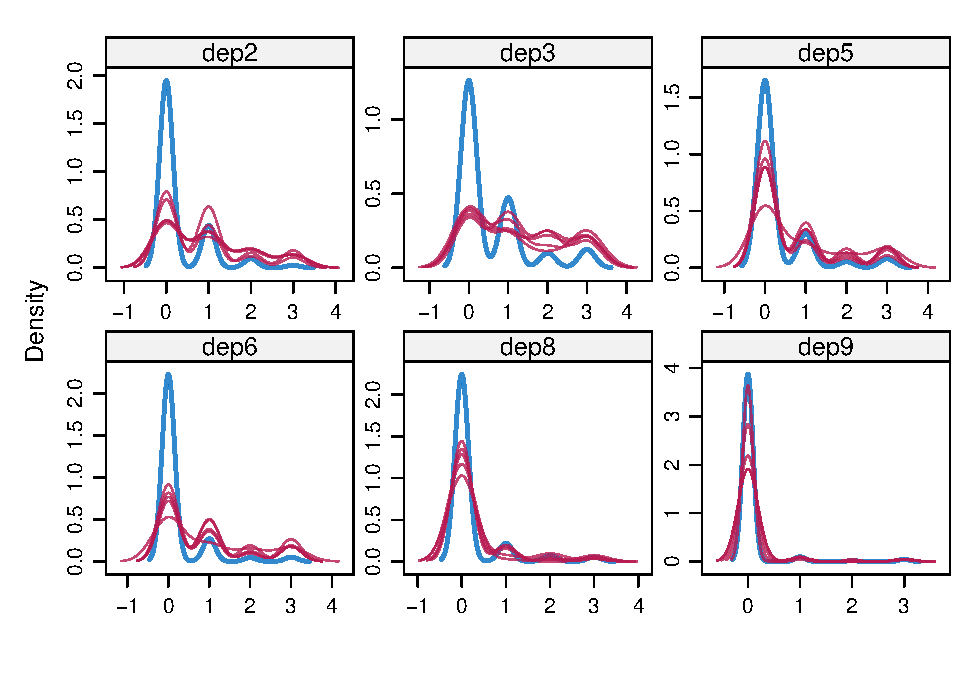
\includegraphics{report_files/figure-latex/dens-multiple-1.pdf}

\includegraphics{report_files/figure-latex/convergence-1.pdf} \includegraphics{report_files/figure-latex/convergence-2.pdf} \includegraphics{report_files/figure-latex/convergence-3.pdf} \includegraphics{report_files/figure-latex/convergence-4.pdf} \includegraphics{report_files/figure-latex/convergence-5.pdf}

\begin{verbatim}
## Warning: Removed 36 rows containing missing values (`geom_line()`).
\end{verbatim}

\includegraphics{report_files/figure-latex/convergence-6.pdf}

\begin{itemize}
\tightlist
\item
  bmi no converge
\item
  weight no intermingle
\item
  remove bmi as pred, justify with table in MDM (no sign predictor for missing vectors of variables of interest)
\end{itemize}

\hypertarget{modelling}{%
\section{Modelling}\label{modelling}}

\hypertarget{interpret}{%
\subsection{Interpretation of the two models}\label{interpret}}

\begin{table}[!h]

\caption{\label{tab:model-compare}Model fit statistics}
\centering
\begin{tabular}[t]{lrrr}
\toprule
model & AIC & BIC & Residual\_Deviance\\
\midrule
\cellcolor{gray!6}{listwise deletion} & \cellcolor{gray!6}{342.6925} & \cellcolor{gray!6}{442.7129} & \cellcolor{gray!6}{286.6925}\\
mean imputation & 576.6865 & 696.0617 & 520.6865\\
\bottomrule
\end{tabular}
\end{table}

\begin{verbatim}
## Waiting for profiling to be done...
## Waiting for profiling to be done...
\end{verbatim}

Two logistic models were created, one for each of the imputed datasets that resulted from both the ad-hoc mean imputation and listwise deletion missing data methods. The interpretation below only includes significant predictors, since most of the model's predictors were non-significant. That said, they are still reported in the model summary tables, as can be seen Table \ref{tab:lw-model} and Table \ref{tab:mi-model} in Appendix A.

Looking at the listwise deletion model, only sex ( \emph{p} \textless0.001) and the marital category \texttt{divorced} ( \emph{p} \textless0.001 ) were significant predictors, whilst all the other predictors (including the intercept) were insignificant. The odds ratio of females drinking regularly compared to males was 0.16{[}0.08, 0.31{]}, meaning they were 0.16 times as likely to drink regularly compared to males. The odds ratio of \texttt{divorced} respondents compared to those who were \texttt{married} was
7.37{[}2.54, 24.98{]},
meaning divorced people were 7.37 times as likely to drink regularly compared to married people.

In the mean imputation model, \texttt{age} (\emph{p} \textless0.001) was also a significant predictor. This was in addition to \texttt{sex} ( \emph{p} \textless0.001) and marital status \texttt{divorced} ( \emph{p} = 0.004 ). Moreover, the \texttt{intercept} ( \emph{p} = 0.001) was also significant. For a unit increase in age the odds ratio of drinking regularly decreases
0.97{[}0.95, 0.99{]}
times. The odds ratio of females drinking regularly compared to males was
0.24{[}0.14, 0.38{]},
meaning they were 0.24 times as likely to drink compared to males. The odds ratio of people with the marital status \texttt{divorced} compared to people with the marital status \texttt{married} was
3.05{[}1.47, 6.69{]},
meaning divorced people were 3.05 times as likely to drink regularly compared to married people. If all predictor variables were in their reference state, the baseline odds ratio was
20.48{[}3.4, 135.96{]}.
Looking at the model fit statistics, the listwise deletion model performed better with a lower AIC, BIC and residual deviance value, as is shown in Table \ref{tab:model-compare}.

\hypertarget{results-comparison-ad-hoc-methods}{%
\subsection{Results comparison ad-hoc methods}\label{results-comparison-ad-hoc-methods}}

Following Section \ref{interpret}, the answer to the research question will differ depending on the ad-hoc method used to treat the missing data. Said difference is comprised of: the number of significant predictors, the odds ratios, standard errors and the fitness statistics. The SE of the mean imputation model was lower than the listwise deletion model, which can be see in Table \ref{tab:mi-model} and \ref{tab:lw-model}.

It was concluded that the missing data treating methods caused biased results within each model, since these methods assume the missingness to be MCAR. This assumption does not hold, in case the data is assumed to be MAR - as was described in Section \ref{MDM}. In the specific case of logistic regression - which was utilised in this study - listwise deletion could still give unbiased results even if the missingness isn't MCAR, but only if the missing values are either in the predictor variables or in the outcome variable. From the EDA and missing data specification it was observed that both predictor \emph{and} outcome variables contained missing data, hence the results were biased as well.

When listwise deletion is used on a dataset where the missingness isn't MCAR, it will result in a bias in the regression coefficients, with standard errors that are too large. As the models in this study were logistic regression models, the regression coefficients were transformed into odds ratios instead. Another negative of listwise deletion is that it is wasteful, a lot of data goes unused. This is also the case in this study, as 263 out of a total of 525 cases were deleted or in other words only half the cases were used. This might explain why the listwise deletion model has a lower \(D\) value; there is just a lot less data that might not fit in the model. Another consequence of removing so much data from the dataset is that it becomes more difficult to find effects, this is a possible explanation for why the listwise deletion model had less significant predictors.

Using mean imputation on a dataset where the missingness isn't MCAR will give biased results and underestimated standard errors. It is indeed the case that the standard errors in the mean imputation model are lower than those in the listwise deletion model. As listwise deletion usually overestimates the standard errors, the real values are probably somewhere in between.

So as both methods were used on data where the missingness wasn't MCAR, the created models were biased in multiple ways.

\hypertarget{conclusion}{%
\section{Conclusion}\label{conclusion}}

The research question was \textbf{To what extent can the occurrence of regular alcohol consumption (12 or more in a year) be predicted by the variables: depression level, age, sex, ethnicity, marital status and household income?} Here, it was expected that sex \texttt{male}, ethnicity \texttt{non-hispanic\_white} and marital status \texttt{married} would exhibit a positive relation with drinking regularly, whilst age and depression would have a negative relation with said outcome variable.

The resulting listwise deletion model - using a logistic regression approach - only had \texttt{sex} and marital status \texttt{divorced} (in reference to \texttt{married}) as significant predictors. Using this ad-hoc method, no significant relation between the predictors \texttt{depression} and \texttt{ethnicity} and the outcome variable \texttt{drink\_regularly} could be deduced. Additionally, \texttt{divorced} was positively related to drinking regularly, which goes against the expectation of categories other than \texttt{married} exhibiting a negative relation with the outcome. The model did suggest that \texttt{male} respondents are more likely to drink regularly than \texttt{female} participants, and can therefore be used to predict alcohol consumption.

As for the mean imputation model, the results similarly suggested non-significant predictors for \texttt{ethnicity} and \texttt{depression}. \texttt{age} was significant, as opposed to in the listwise deletion model - this was in addition to the other significant predictors, those being the married status \texttt{divorced} and \texttt{sex}. Once again, the model aligned with expectations of \texttt{male} respondents drinking more regularly. \texttt{age} also showed a negative relation with the outcome, albeit a small decrease per unit change of \texttt{age}. Similar to the previous model, \texttt{divorced} showed an unexected positive behaviour with the outcome variable.

Overall, it was concluded from both models that \texttt{depression} and \texttt{ethnicity} cannot be used to predict whether a case is drinking regularly. Marital status is a valid predictor, although its relation does not align with research previously done by others. Whether \texttt{age} can be used as a predictor, depends on the ad-hoc method used to treat missing data. Lastly, the coefficients of significant predictors in both models differed greatly. The coefficient of \texttt{divorced} in the listwise deletion model exceeded the mean imputation variant twofold.

\newpage

\hypertarget{references}{%
\section{References}\label{references}}

\hypertarget{refs}{}
\begin{CSLReferences}{1}{0}
\leavevmode\vadjust pre{\hypertarget{ref-FIMD}{}}%
Buuren, Stef van. 2018. \emph{Flexible Imputation of Missing Data}. 2nd ed. Chapman \& Hall/CRC.

\leavevmode\vadjust pre{\hypertarget{ref-garnett}{}}%
Garnett, Claire, Sabrina Kastaun, Jamie Brown, and Daniel Kotz. 2022. {``Alcohol Consumption and Associations with Sociodemographic and Health-Related Characteristics in Germany: A Population Survey.''} \emph{Addictive Behaviors} 125 (February): 107159. \url{https://doi.org/10.1016/j.addbeh.2021.107159}.

\leavevmode\vadjust pre{\hypertarget{ref-GBD}{}}%
GBD 2016 Alcohol Collaborators. 2018. {``Alcohol Use and Burden for 195 Countries and Territories, 1990--2016: A Systematic Analysis for the Global Burden of Disease Study 2016.''} \emph{Lancet} 392 (10152): 1015--35. \url{https://doi.org/10.1016/s0140-6736(18)31310-2}.

\leavevmode\vadjust pre{\hypertarget{ref-vtab}{}}%
Huntington-Klein, Nick. 2023. \emph{Vtable: Variable Table for Variable Documentation}. \url{https://CRAN.R-project.org/package=vtable}.

\leavevmode\vadjust pre{\hypertarget{ref-Little_1986}{}}%
Little, Roderick J. 1986. {``A Test of Missing Completely at Random for Multivariate Data with Missing Values.''} \emph{Journal of the American Statistical Association} 83 (404): 1198--1202. \url{https://doi.org/10.1080/01621459.1988.10478722}.

\leavevmode\vadjust pre{\hypertarget{ref-moore}{}}%
Moore, Alison A., Robert Gould, David B. Reuben, Gail A. Greendale, M. Kallin Carter, Kefei Zhou, and Arun Karlamangla. 2005. {``Longitudinal Patterns and Predictors of Alcohol Consumption in the United States.''} \emph{American Journal of Public Health} 95 (3): 458--64. \url{https://doi.org/10.2105/ajph.2003.019471}.

\leavevmode\vadjust pre{\hypertarget{ref-ggmice}{}}%
Oberman, Hanne. 2024. \emph{Ggmice: Visualizations for 'Mice' with 'Ggplot2'}. \url{https://github.com/amices/ggmice}.

\leavevmode\vadjust pre{\hypertarget{ref-Rversion}{}}%
R Core Team. 2023. \emph{R: A Language and Environment for Statistical Computing}. Vienna, Austria: R Foundation for Statistical Computing. \url{https://www.R-project.org/}.

\leavevmode\vadjust pre{\hypertarget{ref-gtsummary}{}}%
Sjoberg, Daniel D., Karissa Whiting, Michael Curry, Jessica A. Lavery, and Joseph Larmarange. 2021. {``Reproducible Summary Tables with the Gtsummary Package.''} \emph{{The R Journal}} 13: 570--80. \url{https://doi.org/10.32614/RJ-2021-053}.

\leavevmode\vadjust pre{\hypertarget{ref-Soetewey}{}}%
Soetewey, Antoine. n.d. {``Chi-Square Test of Independence in r.''} \emph{Stats and R}. \url{https://statsandr.com/blog/chi-square-test-of-independence-in-r/\#chi-square-test-of-independence-in-r}.

\leavevmode\vadjust pre{\hypertarget{ref-nan}{}}%
Tierney, Nicholas, and Dianne Cook. 2023. {``Expanding Tidy Data Principles to Facilitate Missing Data Exploration, Visualization and Assessment of Imputations.''} \emph{Journal of Statistical Software} 105 (7): 1--31. \url{https://doi.org/10.18637/jss.v105.i07}.

\leavevmode\vadjust pre{\hypertarget{ref-mice}{}}%
van Buuren, Stef, and Karin Groothuis-Oudshoorn. 2011. {``{mice}: Multivariate Imputation by Chained Equations in r.''} \emph{Journal of Statistical Software} 45 (3): 1--67. \url{https://doi.org/10.18637/jss.v045.i03}.

\leavevmode\vadjust pre{\hypertarget{ref-tidyverse}{}}%
Wickham, Hadley, Mara Averick, Jennifer Bryan, Winston Chang, Lucy D'Agostino McGowan, Romain François, Garrett Grolemund, et al. 2019. {``Welcome to the {tidyverse}.''} \emph{Journal of Open Source Software} 4 (43): 1686. \url{https://doi.org/10.21105/joss.01686}.

\leavevmode\vadjust pre{\hypertarget{ref-enders}{}}%
Wu, Wei, Fan Jia, and Craig Enders. 2015. {``A Comparison of Imputation Strategies for Ordinal Missing Data on Likert Scale Variables.''} \emph{Multivariate Behavioral Research} 50 (5): 484--503. \url{https://doi.org/10.1080/00273171.2015.1022644}.

\leavevmode\vadjust pre{\hypertarget{ref-kables}{}}%
Zhu, Hao. 2021. \emph{kableExtra: Construct Complex Table with 'Kable' and Pipe Syntax}. \url{https://CRAN.R-project.org/package=kableExtra}.

\end{CSLReferences}

\hypertarget{appendix-appendix}{%
\appendix}


\hypertarget{vartabfull}{%
\section{Appendix}\label{vartabfull}}

\begin{table}[!h]

\caption{\label{tab:full-vars-desc}Variable descriptions}
\centering
\resizebox{\linewidth}{!}{
\begin{tabular}[t]{lllllll}
\toprule
Role & Variable & Further.Description & Name & Type & Characteristics & Target\\
\midrule
\cellcolor{gray!6}{Outcome} & \cellcolor{gray!6}{Drink regularly} & \cellcolor{gray!6}{at least 12 drinks in a year} & \cellcolor{gray!6}{drink\_regularly} & \cellcolor{gray!6}{Categorical} & \cellcolor{gray!6}{Binary, yes and no} & \cellcolor{gray!6}{m/f, age 20-150}\\
Predictor & Sex &  & sex & Categorical & Binary, male and female & m/f, age 0-150\\
\cellcolor{gray!6}{Predictor} & \cellcolor{gray!6}{Age} & \cellcolor{gray!6}{years at screening} & \cellcolor{gray!6}{age} & \cellcolor{gray!6}{Numeric} & \cellcolor{gray!6}{Discrete} & \cellcolor{gray!6}{m/f, age 0-150}\\
Predictor & Ethnicity &  & ethnicity & Categorical & Nominal, 5 categories & m/f, age 0-150\\
\cellcolor{gray!6}{Predictor} & \cellcolor{gray!6}{Education} & \cellcolor{gray!6}{} & \cellcolor{gray!6}{marital} & \cellcolor{gray!6}{Categorical} & \cellcolor{gray!6}{Nominal, 5 categories} & \cellcolor{gray!6}{m/f, age 20-150}\\
\addlinespace
Predictor & Marital status &  & marital & Categorical & Nominal, 5 categories & m/f, age 20-150\\
\cellcolor{gray!6}{Predictor} & \cellcolor{gray!6}{household income} & \cellcolor{gray!6}{annual in USD} & \cellcolor{gray!6}{household\_income} & \cellcolor{gray!6}{Categorical} & \cellcolor{gray!6}{Nominal, 12 categories} & \cellcolor{gray!6}{m/f, age 0-150}\\
Predictor & No interest in activity &  & dep1 & Categorical & Ordinal, 1-3 scale & m/f, age 18-150\\
\cellcolor{gray!6}{Predictor} & \cellcolor{gray!6}{Feeling depressed} & \cellcolor{gray!6}{} & \cellcolor{gray!6}{dep2} & \cellcolor{gray!6}{Categorical} & \cellcolor{gray!6}{Ordinal, 1-3 scale} & \cellcolor{gray!6}{m/f, age 18-150}\\
Predictor & Sleeping issues &  & dep3 & Categorical & Ordinal, 1-3 scale & m/f, age 18-150\\
\addlinespace
\cellcolor{gray!6}{Predictor} & \cellcolor{gray!6}{Feeling tired} & \cellcolor{gray!6}{} & \cellcolor{gray!6}{dep4} & \cellcolor{gray!6}{Categorical} & \cellcolor{gray!6}{Ordinal, 1-3 scale} & \cellcolor{gray!6}{m/f, age 18-150}\\
Predictor & Eating issues &  & dep5 & Categorical & Ordinal, 1-3 scale & m/f, age 18-150\\
\cellcolor{gray!6}{Predictor} & \cellcolor{gray!6}{Feeling bad about yourself} & \cellcolor{gray!6}{} & \cellcolor{gray!6}{dep6} & \cellcolor{gray!6}{Categorical} & \cellcolor{gray!6}{Ordinal, 1-3 scale} & \cellcolor{gray!6}{m/f, age 18-150}\\
Predictor & Concentrating issues &  & dep7 & Categorical & Ordinal, 1-3 scale & m/f, age 18-150\\
\cellcolor{gray!6}{Predictor} & \cellcolor{gray!6}{Moving and speaking issues} & \cellcolor{gray!6}{} & \cellcolor{gray!6}{dep8} & \cellcolor{gray!6}{Categorical} & \cellcolor{gray!6}{Ordinal, 1-3 scale} & \cellcolor{gray!6}{m/f, age 18-150}\\
\addlinespace
Predictor & Suicidial thoughts &  & dep9 & Categorical & Ordinal, 1-3 scale & m/f, age 18-150\\
\cellcolor{gray!6}{Imputation} & \cellcolor{gray!6}{Household size} & \cellcolor{gray!6}{number of people} & \cellcolor{gray!6}{household\_size} & \cellcolor{gray!6}{Numeric} & \cellcolor{gray!6}{Discrete} & \cellcolor{gray!6}{m/f, age 0-150}\\
Imputation & Weight & in kg & weight & Numeric & Continious & m/f, age 0-150\\
\cellcolor{gray!6}{Imputation} & \cellcolor{gray!6}{Height} & \cellcolor{gray!6}{standing in cm} & \cellcolor{gray!6}{height} & \cellcolor{gray!6}{Numeric} & \cellcolor{gray!6}{Continious} & \cellcolor{gray!6}{m/f, age 2-150}\\
Imputation & Body Mass Index & in kg/m\textasciicircum{}2 & bmi & Numeric & Continious & m/f, age 2-150\\
\addlinespace
\cellcolor{gray!6}{Imputation} & \cellcolor{gray!6}{Pulse} & \cellcolor{gray!6}{beats per minute} & \cellcolor{gray!6}{pulse} & \cellcolor{gray!6}{Numeric} & \cellcolor{gray!6}{Discrete} & \cellcolor{gray!6}{m/f, age 8-150}\\
Imputation & Systolic blood pressure & 1st reading, in mm Hg & bp\_sys1 & Numeric & Discrete & m/f, age 8-150\\
\cellcolor{gray!6}{Imputation} & \cellcolor{gray!6}{Diastolic blood pressure} & \cellcolor{gray!6}{1st reading, in mm Hg} & \cellcolor{gray!6}{bp\_dia1} & \cellcolor{gray!6}{Numeric} & \cellcolor{gray!6}{Discrete} & \cellcolor{gray!6}{m/f, age 8-150}\\
Imputation & Systolic blood pressure & 2nd reading, in mm Hg & bp\_sys2 & Numeric & Discrete & m/f, age 8-150\\
\cellcolor{gray!6}{Imputation} & \cellcolor{gray!6}{Diastolic blood pressure} & \cellcolor{gray!6}{2nd reading, in mm Hg} & \cellcolor{gray!6}{bp\_dia2} & \cellcolor{gray!6}{Numeric} & \cellcolor{gray!6}{Discrete} & \cellcolor{gray!6}{m/f, age 8-150}\\
\addlinespace
Imputation & Vigorous work activity &  & vig\_work & Categorical & Binary, yes and no & m/f, age 12-150\\
\cellcolor{gray!6}{Imputation} & \cellcolor{gray!6}{Moderate work activity} & \cellcolor{gray!6}{} & \cellcolor{gray!6}{mod\_work} & \cellcolor{gray!6}{Categorical} & \cellcolor{gray!6}{Binary, yes and no} & \cellcolor{gray!6}{m/f, age 12-150}\\
Imputation & Walking or cycling &  & walk\_cycle & Categorical & Binary, yes and no & m/f, age 12-150\\
\cellcolor{gray!6}{Imputation} & \cellcolor{gray!6}{Vigorous sport activity} & \cellcolor{gray!6}{} & \cellcolor{gray!6}{vig\_rec} & \cellcolor{gray!6}{Categorical} & \cellcolor{gray!6}{Binary, yes and no} & \cellcolor{gray!6}{m/f, age 12-150}\\
Imputation & Moderate sport activity &  & mod\_rec & Categorical & Binary, yes and no & m/f, age 12-150\\
\addlinespace
\cellcolor{gray!6}{Imputation} & \cellcolor{gray!6}{Sedentary activity} & \cellcolor{gray!6}{in minutes} & \cellcolor{gray!6}{time\_sed} & \cellcolor{gray!6}{Numeric} & \cellcolor{gray!6}{Discrete} & \cellcolor{gray!6}{m/f, age 12-150}\\
Imputation & Number of sex & in a year & n\_sex\_year & Categorical & Nominal, 7 categories & m/f, age 20-59\\
\cellcolor{gray!6}{Imputation} & \cellcolor{gray!6}{Frequency of unsafe sex} & \cellcolor{gray!6}{in a year} & \cellcolor{gray!6}{n\_unsafe\_sex\_year} & \cellcolor{gray!6}{Categorical} & \cellcolor{gray!6}{Nominal, 5 categories} & \cellcolor{gray!6}{m/f, age 20-59}\\
Imputation & Number of days drinking aclohol &  & days\_drinking & Numeric & Discrete & m/f, age 20-150\\
\bottomrule
\end{tabular}}
\end{table}

\newpage

\hypertarget{apEDA}{%
\section{Appendix}\label{apEDA}}

\begin{table}

\caption{\label{tab:data-sum}Summary statistics of variables of intrest}
\centering
\begin{tabular}[t]{llllllll}
\toprule
Variable & N & Mean & Std. Dev. & Min & Pctl. 25 & Pctl. 75 & Max\\
\midrule
drink\_regularly & 446 &  &  &  &  &  & \\
... no & 139 & 31\% &  &  &  &  & \\
... yes & 307 & 69\% &  &  &  &  & \\
sex & 525 &  &  &  &  &  & \\
... male & 254 & 48\% &  &  &  &  & \\
\addlinespace
... female & 271 & 52\% &  &  &  &  & \\
age & 525 & 45 & 14 & 20 & 33 & 57 & 69\\
ethnicity & 525 &  &  &  &  &  & \\
... mexican\_american & 95 & 18\% &  &  &  &  & \\
... other\_hispanic & 61 & 12\% &  &  &  &  & \\
\addlinespace
... non-hispanic\_white & 220 & 42\% &  &  &  &  & \\
... non-hispanic\_black & 124 & 24\% &  &  &  &  & \\
... other & 25 & 5\% &  &  &  &  & \\
education & 525 &  &  &  &  &  & \\
... no\_high\_school & 58 & 11\% &  &  &  &  & \\
\addlinespace
... some\_high\_school & 101 & 19\% &  &  &  &  & \\
... high\_school\_grad & 123 & 23\% &  &  &  &  & \\
... some\_college & 155 & 30\% &  &  &  &  & \\
... college\_grad & 88 & 17\% &  &  &  &  & \\
marital & 525 &  &  &  &  &  & \\
\addlinespace
... married & 279 & 53\% &  &  &  &  & \\
... widowed & 19 & 4\% &  &  &  &  & \\
... divorced & 67 & 13\% &  &  &  &  & \\
... separated & 14 & 3\% &  &  &  &  & \\
... never\_married & 102 & 19\% &  &  &  &  & \\
\addlinespace
... living\_with\_partner & 44 & 8\% &  &  &  &  & \\
income & 525 &  &  &  &  &  & \\
... 0:4999 & 13 & 2\% &  &  &  &  & \\
... 5000:9999 & 24 & 5\% &  &  &  &  & \\
... 10000:14999 & 45 & 9\% &  &  &  &  & \\
\addlinespace
... 15000:19999 & 40 & 8\% &  &  &  &  & \\
... 20000:24999 & 52 & 10\% &  &  &  &  & \\
... 25000:34999 & 59 & 11\% &  &  &  &  & \\
... 35000:44999 & 51 & 10\% &  &  &  &  & \\
... 45000:54999 & 44 & 8\% &  &  &  &  & \\
\addlinespace
... 55000:64999 & 35 & 7\% &  &  &  &  & \\
... 65000:74999 & 37 & 7\% &  &  &  &  & \\
... 75000:99999 & 49 & 9\% &  &  &  &  & \\
... 100000+ & 76 & 14\% &  &  &  &  & \\
dep1 & 525 & 0.41 & 0.79 & 0 & 0 & 1 & 3\\
\addlinespace
dep2 & 394 & 0.28 & 0.58 & 0 & 0 & 0 & 3\\
dep3 & 394 & 0.53 & 0.86 & 0 & 0 & 1 & 3\\
dep4 & 525 & 0.76 & 0.9 & 0 & 0 & 1 & 3\\
dep5 & 394 & 0.31 & 0.7 & 0 & 0 & 0 & 3\\
dep6 & 394 & 0.2 & 0.56 & 0 & 0 & 0 & 3\\
\addlinespace
dep7 & 525 & 0.32 & 0.71 & 0 & 0 & 0 & 3\\
dep8 & 473 & 0.2 & 0.59 & 0 & 0 & 0 & 3\\
dep9 & 449 & 0.067 & 0.37 & 0 & 0 & 0 & 3\\
\bottomrule
\end{tabular}
\end{table}

\begin{table}

\caption{\label{tab:imp-data-sum}Summary statistics of varaibles used only for imputation}
\centering
\begin{tabular}[t]{llllllll}
\toprule
Variable & N & Mean & Std. Dev. & Min & Pctl. 25 & Pctl. 75 & Max\\
\midrule
household\_size & 525 & 3.4 & 1.6 & 1 & 2 & 4 & 7\\
weight & 446 & 81 & 20 & 42 & 65 & 92 & 164\\
height & 414 & 167 & 10 & 144 & 160 & 174 & 204\\
bmi & 207 & 29 & 6.6 & 14 & 24 & 33 & 51\\
pulse & 525 & 74 & 13 & 46 & 66 & 82 & 136\\
\addlinespace
bp\_sys1 & 525 & 122 & 18 & 84 & 112 & 132 & 218\\
bp\_dia1 & 525 & 72 & 12 & 26 & 64 & 80 & 114\\
bp\_sys2 & 420 & 120 & 17 & 76 & 108 & 128 & 204\\
bp\_dia2 & 420 & 71 & 11 & 28 & 64 & 76 & 106\\
vig\_work & 525 &  &  &  &  &  & \\
\addlinespace
... yes & 111 & 21\% &  &  &  &  & \\
... no & 414 & 79\% &  &  &  &  & \\
mod\_work & 525 &  &  &  &  &  & \\
... yes & 215 & 41\% &  &  &  &  & \\
... no & 310 & 59\% &  &  &  &  & \\
\addlinespace
walk\_cycle & 525 &  &  &  &  &  & \\
... yes & 144 & 27\% &  &  &  &  & \\
... no & 381 & 73\% &  &  &  &  & \\
vig\_rec & 420 &  &  &  &  &  & \\
... yes & 95 & 23\% &  &  &  &  & \\
\addlinespace
... no & 325 & 77\% &  &  &  &  & \\
mod\_rec & 420 &  &  &  &  &  & \\
... yes & 165 & 39\% &  &  &  &  & \\
... no & 255 & 61\% &  &  &  &  & \\
time\_sed & 525 & 292 & 199 & 5 & 120 & 420 & 1080\\
\addlinespace
n\_sex\_year & 525 &  &  &  &  &  & \\
... 0 & 131 & 25\% &  &  &  &  & \\
... 1 & 22 & 4\% &  &  &  &  & \\
... 2:11 & 105 & 20\% &  &  &  &  & \\
... 12:51 & 148 & 28\% &  &  &  &  & \\
\addlinespace
... 52:103 & 73 & 14\% &  &  &  &  & \\
... 104:364 & 43 & 8\% &  &  &  &  & \\
... 365+ & 3 & 1\% &  &  &  &  & \\
n\_unsafe\_sex\_year & 394 &  &  &  &  &  & \\
... never & 203 & 52\% &  &  &  &  & \\
\addlinespace
... less than half & 39 & 10\% &  &  &  &  & \\
... about half & 11 & 3\% &  &  &  &  & \\
... more than half & 15 & 4\% &  &  &  &  & \\
... always & 126 & 32\% &  &  &  &  & \\
days\_drinking & 525 & 50 & 84 & 0 & 1 & 52 & 364\\
\bottomrule
\end{tabular}
\end{table}

\begin{verbatim}
## 
## Attaching package: 'reshape2'
\end{verbatim}

\begin{verbatim}
## The following object is masked from 'package:tidyr':
## 
##     smiths
\end{verbatim}

\includegraphics{report_files/figure-latex/tile-cor-1.pdf}
\includegraphics{report_files/figure-latex/box-drink-1.pdf}

\newpage

\hypertarget{apmissing}{%
\section{Appendix}\label{apmissing}}

\begin{table}[!h]

\caption{\label{tab:imp-t-test}Dependency t-test: mean comparison in numerical variables across missing values and observed values in the other variables}
\centering
\resizebox{\linewidth}{!}{
\begin{tabular}[t]{lllll}
\toprule
numerical variable & missing drink\_regularly & missing dep2/3/5/6 & missing dep8 & missing dep9\\
\midrule
\cellcolor{gray!6}{days\_drinking} & \cellcolor{gray!6}{t = -4.42, pVal = 2.7e-05} & \cellcolor{gray!6}{t = -3.05, pVal = 0.00261} & \cellcolor{gray!6}{t = -1.48, pVal = 0.145} & \cellcolor{gray!6}{t = 0.0761, pVal = 0.94}\\
time\_sed & t = 0.308, pVal = 0.759 & t = -0.593, pVal = 0.554 & t = -0.88, pVal = 0.382 & t = 0.135, pVal = 0.893\\
\cellcolor{gray!6}{bp\_dia2} & \cellcolor{gray!6}{t = 2.55, pVal = 0.0125} & \cellcolor{gray!6}{t = 0.359, pVal = 0.72} & \cellcolor{gray!6}{t = -1.85, pVal = 0.0697} & \cellcolor{gray!6}{t = 1.75, pVal = 0.0844}\\
bp\_sys2 & t = 2.28, pVal = 0.0249 & t = -0.0284, pVal = 0.977 & t = -2.3, pVal = 0.026 & t = 0.675, pVal = 0.502\\
\cellcolor{gray!6}{bp\_dia1} & \cellcolor{gray!6}{t = 2.59, pVal = 0.0111} & \cellcolor{gray!6}{t = 0.837, pVal = 0.404} & \cellcolor{gray!6}{t = -0.816, pVal = 0.418} & \cellcolor{gray!6}{t = 1.49, pVal = 0.14}\\
\addlinespace
bp\_sys1 & t = 4.09, pVal = 7.67e-05 & t = 1.4, pVal = 0.162 & t = -2.32, pVal = 0.0236 & t = 1.1, pVal = 0.274\\
\cellcolor{gray!6}{pulse} & \cellcolor{gray!6}{t = -1.98, pVal = 0.0499} & \cellcolor{gray!6}{t = -0.94, pVal = 0.349} & \cellcolor{gray!6}{t = 1.25, pVal = 0.215} & \cellcolor{gray!6}{t = -0.478, pVal = 0.634}\\
bmi & t = -0.146, pVal = 0.884 & t = 1.48, pVal = 0.141 & t = -1.52, pVal = 0.141 & t = -0.209, pVal = 0.836\\
\cellcolor{gray!6}{height} & \cellcolor{gray!6}{t = -3.91, pVal = 0.000181} & \cellcolor{gray!6}{t = -1.71, pVal = 0.0885} & \cellcolor{gray!6}{t = 0.398, pVal = 0.692} & \cellcolor{gray!6}{t = 0.848, pVal = 0.399}\\
weight & t = 0.808, pVal = 0.421 & t = 1.2, pVal = 0.233 & t = 0.135, pVal = 0.893 & t = 0.32, pVal = 0.75\\
\addlinespace
\cellcolor{gray!6}{household\_size} & \cellcolor{gray!6}{t = -1.72, pVal = 0.0882} & \cellcolor{gray!6}{t = -1.2, pVal = 0.231} & \cellcolor{gray!6}{t = -0.604, pVal = 0.548} & \cellcolor{gray!6}{t = -0.904, pVal = 0.368}\\
age & t = 19.3, pVal = 3.1e-45 & t = 1.38, pVal = 0.17 & t = -1.16, pVal = 0.249 & t = -0.884, pVal = 0.379\\
\bottomrule
\end{tabular}}
\end{table}

\begin{Shaded}
\begin{Highlighting}[]
\CommentTok{\# Make a table with outcomes of the chi{-}squared:}
\NormalTok{col1 }\OtherTok{\textless{}{-}} \FunctionTok{c}\NormalTok{(}\StringTok{"vig\_work"}\NormalTok{,}
\StringTok{"mod\_work"}\NormalTok{,}
\StringTok{"walk\_cycle"}\NormalTok{,}
\StringTok{"vig\_rec"}\NormalTok{,}
\StringTok{"mod\_rec"}\NormalTok{,}
\StringTok{"n\_sex\_year"}\NormalTok{,}
\StringTok{"n\_unsafe\_sex\_year"}\NormalTok{)}

\NormalTok{col2 }\OtherTok{\textless{}{-}} \FunctionTok{c}\NormalTok{(}\FunctionTok{dependency\_chitest}\NormalTok{(}\AttributeTok{var =}\NormalTok{ main\_data}\SpecialCharTok{$}\NormalTok{vig\_work, }\AttributeTok{mis\_vector =}\NormalTok{ mdrink), }\FunctionTok{dependency\_chitest}\NormalTok{(}\AttributeTok{var =}\NormalTok{ main\_data}\SpecialCharTok{$}\NormalTok{mod\_work, }\AttributeTok{mis\_vector =}\NormalTok{ mdrink), }\FunctionTok{dependency\_chitest}\NormalTok{(}\AttributeTok{var =}\NormalTok{ main\_data}\SpecialCharTok{$}\NormalTok{walk\_cycle, }\AttributeTok{mis\_vector =}\NormalTok{ mdrink), }\FunctionTok{dependency\_chitest}\NormalTok{(}\AttributeTok{var =}\NormalTok{ main\_data}\SpecialCharTok{$}\NormalTok{vig\_rec, }\AttributeTok{mis\_vector =}\NormalTok{ mdrink), }\FunctionTok{dependency\_chitest}\NormalTok{(}\AttributeTok{var =}\NormalTok{ main\_data}\SpecialCharTok{$}\NormalTok{mod\_rec, }\AttributeTok{mis\_vector =}\NormalTok{ mdrink), }\FunctionTok{dependency\_chitest}\NormalTok{(}\AttributeTok{var =}\NormalTok{ main\_data}\SpecialCharTok{$}\NormalTok{n\_sex\_year, }\AttributeTok{mis\_vector =}\NormalTok{ mdrink), }\FunctionTok{dependency\_chitest}\NormalTok{(}\AttributeTok{var =}\NormalTok{ main\_data}\SpecialCharTok{$}\NormalTok{n\_unsafe\_sex\_year, }\AttributeTok{mis\_vector =}\NormalTok{ mdrink))}
\end{Highlighting}
\end{Shaded}

\begin{verbatim}
## Warning in chisq.test(table(var, mis_vector)): Chi-squared approximation may be
## incorrect

## Warning in chisq.test(table(var, mis_vector)): Chi-squared approximation may be
## incorrect
\end{verbatim}

\begin{Shaded}
\begin{Highlighting}[]
\NormalTok{col3 }\OtherTok{\textless{}{-}} \FunctionTok{c}\NormalTok{(}\FunctionTok{dependency\_chitest}\NormalTok{(}\AttributeTok{var =}\NormalTok{ main\_data}\SpecialCharTok{$}\NormalTok{vig\_work, }\AttributeTok{mis\_vector =}\NormalTok{ mdep2), }\FunctionTok{dependency\_chitest}\NormalTok{(}\AttributeTok{var =}\NormalTok{ main\_data}\SpecialCharTok{$}\NormalTok{mod\_work, }\AttributeTok{mis\_vector =}\NormalTok{  mdep2), }\FunctionTok{dependency\_chitest}\NormalTok{(}\AttributeTok{var =}\NormalTok{ main\_data}\SpecialCharTok{$}\NormalTok{walk\_cycle, }\AttributeTok{mis\_vector =}\NormalTok{ mdep2), }\FunctionTok{dependency\_chitest}\NormalTok{(}\AttributeTok{var =}\NormalTok{ main\_data}\SpecialCharTok{$}\NormalTok{vig\_rec, }\AttributeTok{mis\_vector =}\NormalTok{  mdep2), }\FunctionTok{dependency\_chitest}\NormalTok{(}\AttributeTok{var =}\NormalTok{ main\_data}\SpecialCharTok{$}\NormalTok{mod\_rec, }\AttributeTok{mis\_vector =}\NormalTok{  mdep2), }\FunctionTok{dependency\_chitest}\NormalTok{(}\AttributeTok{var =}\NormalTok{ main\_data}\SpecialCharTok{$}\NormalTok{n\_sex\_year, }\AttributeTok{mis\_vector =}\NormalTok{  mdep2), }\FunctionTok{dependency\_chitest}\NormalTok{(}\AttributeTok{var =}\NormalTok{ main\_data}\SpecialCharTok{$}\NormalTok{n\_unsafe\_sex\_year, }\AttributeTok{mis\_vector =}\NormalTok{  mdep2))}
\end{Highlighting}
\end{Shaded}

\begin{verbatim}
## Warning in chisq.test(table(var, mis_vector)): Chi-squared approximation may be
## incorrect

## Warning in chisq.test(table(var, mis_vector)): Chi-squared approximation may be
## incorrect
\end{verbatim}

\begin{Shaded}
\begin{Highlighting}[]
\NormalTok{col4 }\OtherTok{\textless{}{-}} \FunctionTok{c}\NormalTok{(}\FunctionTok{dependency\_chitest}\NormalTok{(}\AttributeTok{var =}\NormalTok{ main\_data}\SpecialCharTok{$}\NormalTok{vig\_work, }\AttributeTok{mis\_vector =}\NormalTok{ mdep8), }\FunctionTok{dependency\_chitest}\NormalTok{(}\AttributeTok{var =}\NormalTok{ main\_data}\SpecialCharTok{$}\NormalTok{mod\_work, }\AttributeTok{mis\_vector =}\NormalTok{  mdep8), }\FunctionTok{dependency\_chitest}\NormalTok{(}\AttributeTok{var =}\NormalTok{ main\_data}\SpecialCharTok{$}\NormalTok{walk\_cycle, }\AttributeTok{mis\_vector =}\NormalTok{  mdep8), }\FunctionTok{dependency\_chitest}\NormalTok{(}\AttributeTok{var =}\NormalTok{ main\_data}\SpecialCharTok{$}\NormalTok{vig\_rec, }\AttributeTok{mis\_vector =}\NormalTok{  mdep8), }\FunctionTok{dependency\_chitest}\NormalTok{(}\AttributeTok{var =}\NormalTok{ main\_data}\SpecialCharTok{$}\NormalTok{mod\_rec, }\AttributeTok{mis\_vector =}\NormalTok{  mdep8), }\FunctionTok{dependency\_chitest}\NormalTok{(}\AttributeTok{var =}\NormalTok{ main\_data}\SpecialCharTok{$}\NormalTok{n\_sex\_year, }\AttributeTok{mis\_vector =}\NormalTok{  mdep8), }\FunctionTok{dependency\_chitest}\NormalTok{(}\AttributeTok{var =}\NormalTok{ main\_data}\SpecialCharTok{$}\NormalTok{n\_unsafe\_sex\_year, }\AttributeTok{mis\_vector =}\NormalTok{  mdep8) )}
\end{Highlighting}
\end{Shaded}

\begin{verbatim}
## Warning in chisq.test(table(var, mis_vector)): Chi-squared approximation may be
## incorrect

## Warning in chisq.test(table(var, mis_vector)): Chi-squared approximation may be
## incorrect
\end{verbatim}

\begin{Shaded}
\begin{Highlighting}[]
\NormalTok{col5 }\OtherTok{\textless{}{-}} \FunctionTok{c}\NormalTok{(}\FunctionTok{dependency\_chitest}\NormalTok{(}\AttributeTok{var =}\NormalTok{ main\_data}\SpecialCharTok{$}\NormalTok{vig\_work, }\AttributeTok{mis\_vector =}\NormalTok{ mdep9), }\FunctionTok{dependency\_chitest}\NormalTok{(}\AttributeTok{var =}\NormalTok{ main\_data}\SpecialCharTok{$}\NormalTok{mod\_work, }\AttributeTok{mis\_vector =}\NormalTok{  mdep9), }\FunctionTok{dependency\_chitest}\NormalTok{(}\AttributeTok{var =}\NormalTok{ main\_data}\SpecialCharTok{$}\NormalTok{walk\_cycle, }\AttributeTok{mis\_vector =}\NormalTok{  mdep9), }\FunctionTok{dependency\_chitest}\NormalTok{(}\AttributeTok{var =}\NormalTok{ main\_data}\SpecialCharTok{$}\NormalTok{vig\_rec, }\AttributeTok{mis\_vector =}\NormalTok{  mdep9), }\FunctionTok{dependency\_chitest}\NormalTok{(}\AttributeTok{var =}\NormalTok{ main\_data}\SpecialCharTok{$}\NormalTok{mod\_rec, }\AttributeTok{mis\_vector =}\NormalTok{  mdep9), }\FunctionTok{dependency\_chitest}\NormalTok{(}\AttributeTok{var =}\NormalTok{ main\_data}\SpecialCharTok{$}\NormalTok{n\_sex\_year, }\AttributeTok{mis\_vector =}\NormalTok{  mdep9), }\FunctionTok{dependency\_chitest}\NormalTok{(}\AttributeTok{var =}\NormalTok{ main\_data}\SpecialCharTok{$}\NormalTok{n\_unsafe\_sex\_year, }\AttributeTok{mis\_vector =}\NormalTok{  mdep9))}
\end{Highlighting}
\end{Shaded}

\begin{verbatim}
## Warning in chisq.test(table(var, mis_vector)): Chi-squared approximation may be
## incorrect

## Warning in chisq.test(table(var, mis_vector)): Chi-squared approximation may be
## incorrect
\end{verbatim}

\begin{Shaded}
\begin{Highlighting}[]
\NormalTok{table\_test2 }\OtherTok{\textless{}{-}}\FunctionTok{as.data.frame}\NormalTok{(}\FunctionTok{cbind}\NormalTok{(col1, col2, col3, col4, col5))}

\FunctionTok{names}\NormalTok{(table\_test2) }\OtherTok{\textless{}{-}} \FunctionTok{c}\NormalTok{(}\StringTok{"categorical variable"}\NormalTok{, }
    \StringTok{"missing drink\_regularly"}\NormalTok{,}
    \StringTok{"missing dep2/3/5/6"}\NormalTok{,}
    \StringTok{"missing dep8"}\NormalTok{,}
    \StringTok{"missing dep9"}\NormalTok{)}

\FunctionTok{show\_table}\NormalTok{(table\_test2, }\StringTok{"Independency Chi{-}squared test"}\NormalTok{)}
\end{Highlighting}
\end{Shaded}

\begin{table}[!h]

\caption{\label{tab:unnamed-chunk-1}Independency Chi-squared test}
\centering
\resizebox{\linewidth}{!}{
\begin{tabular}[t]{lllll}
\toprule
categorical variable & missing drink\_regularly & missing dep2/3/5/6 & missing dep8 & missing dep9\\
\midrule
\cellcolor{gray!6}{vig\_work} & \cellcolor{gray!6}{X\textasciicircum{}2 = 0.0568, pVal = 0.812} & \cellcolor{gray!6}{X\textasciicircum{}2 = 6.2e-30, pVal = 1} & \cellcolor{gray!6}{X\textasciicircum{}2 = 2.01e-30, pVal = 1} & \cellcolor{gray!6}{X\textasciicircum{}2 = 0.546, pVal = 0.46}\\
mod\_work & X\textasciicircum{}2 = 1.63, pVal = 0.201 & X\textasciicircum{}2 = 0.194, pVal = 0.66 & X\textasciicircum{}2 = 0.429, pVal = 0.512 & X\textasciicircum{}2 = 1.22, pVal = 0.27\\
\cellcolor{gray!6}{walk\_cycle} & \cellcolor{gray!6}{X\textasciicircum{}2 = 1.75, pVal = 0.186} & \cellcolor{gray!6}{X\textasciicircum{}2 = 0.126, pVal = 0.723} & \cellcolor{gray!6}{X\textasciicircum{}2 = 1.12, pVal = 0.289} & \cellcolor{gray!6}{X\textasciicircum{}2 = 5.65e-31, pVal = 1}\\
vig\_rec & X\textasciicircum{}2 = 7.84, pVal = 0.00512 & X\textasciicircum{}2 = 0.00635, pVal = 0.937 & X\textasciicircum{}2 = 0, pVal = 1 & X\textasciicircum{}2 = 2.21, pVal = 0.137\\
\cellcolor{gray!6}{mod\_rec} & \cellcolor{gray!6}{X\textasciicircum{}2 = 0.416, pVal = 0.519} & \cellcolor{gray!6}{X\textasciicircum{}2 = 0.338, pVal = 0.561} & \cellcolor{gray!6}{X\textasciicircum{}2 = 0.111, pVal = 0.739} & \cellcolor{gray!6}{X\textasciicircum{}2 = 0.274, pVal = 0.601}\\
\addlinespace
n\_sex\_year & X\textasciicircum{}2 = 28.9, pVal = 6.3e-05 & X\textasciicircum{}2 = 1.97, pVal = 0.923 & X\textasciicircum{}2 = 8.64, pVal = 0.195 & X\textasciicircum{}2 = 2.72, pVal = 0.843\\
\cellcolor{gray!6}{n\_unsafe\_sex\_year} & \cellcolor{gray!6}{X\textasciicircum{}2 = 18.7, pVal = 0.000888} & \cellcolor{gray!6}{X\textasciicircum{}2 = 7.7, pVal = 0.103} & \cellcolor{gray!6}{X\textasciicircum{}2 = 7.59, pVal = 0.108} & \cellcolor{gray!6}{X\textasciicircum{}2 = 1.56, pVal = 0.816}\\
\bottomrule
\end{tabular}}
\end{table}

\hypertarget{appendix}{%
\section{Appendix}\label{appendix}}

\begin{longtable}[t]{lccc}
\caption{\label{tab:lw-model}Listwise deletion model}\\
\toprule
\textbf{Characteristic} & \textbf{OR} & \textbf{SE} & \textbf{p-value}\\
\midrule
\endfirsthead
\caption[]{\label{tab:lw-model}Listwise deletion model \textit{(continued)}}\\
\toprule
\textbf{Characteristic} & \textbf{OR} & \textbf{SE} & \textbf{p-value}\\
\midrule
\endhead

\endfoot
\bottomrule
\endlastfoot
\cellcolor{gray!15}{(Intercept)} & \cellcolor{gray!15}{6.71} & \cellcolor{gray!15}{1.28} & \cellcolor{gray!15}{0.14}\\
sex &  &  & \\
\cellcolor{gray!15}{\hspace{1em}male} & \cellcolor{gray!15}{—} & \cellcolor{gray!15}{—} & \cellcolor{gray!15}{}\\
\hspace{1em}female & 0.16*** & 0.350 & <0.001\\
\cellcolor{gray!15}{age} & \cellcolor{gray!15}{1.00} & \cellcolor{gray!15}{0.013} & \cellcolor{gray!15}{0.8}\\
ethnicity &  &  & \\
\cellcolor{gray!15}{\hspace{1em}mexican\_american} & \cellcolor{gray!15}{—} & \cellcolor{gray!15}{—} & \cellcolor{gray!15}{}\\
\hspace{1em}other\_hispanic & 1.49 & 0.594 & 0.5\\
\cellcolor{gray!15}{\hspace{1em}non-hispanic\_white} & \cellcolor{gray!15}{1.58} & \cellcolor{gray!15}{0.435} & \cellcolor{gray!15}{0.3}\\
\hspace{1em}non-hispanic\_black & 0.55 & 0.485 & 0.2\\
\cellcolor{gray!15}{\hspace{1em}other} & \cellcolor{gray!15}{1.04} & \cellcolor{gray!15}{0.792} & \cellcolor{gray!15}{>0.9}\\
education &  &  & \\
\cellcolor{gray!15}{\hspace{1em}no\_high\_school} & \cellcolor{gray!15}{—} & \cellcolor{gray!15}{—} & \cellcolor{gray!15}{}\\
\hspace{1em}some\_high\_school & 0.82 & 0.582 & 0.7\\
\cellcolor{gray!15}{\hspace{1em}high\_school\_grad} & \cellcolor{gray!15}{1.30} & \cellcolor{gray!15}{0.589} & \cellcolor{gray!15}{0.7}\\
\hspace{1em}some\_college & 1.05 & 0.604 & >0.9\\
\cellcolor{gray!15}{\hspace{1em}college\_grad} & \cellcolor{gray!15}{1.66} & \cellcolor{gray!15}{0.647} & \cellcolor{gray!15}{0.4}\\
marital &  &  & \\
\cellcolor{gray!15}{\hspace{1em}married} & \cellcolor{gray!15}{—} & \cellcolor{gray!15}{—} & \cellcolor{gray!15}{}\\
\hspace{1em}widowed & 1.37 & 0.711 & 0.7\\
\cellcolor{gray!15}{\hspace{1em}divorced} & \cellcolor{gray!15}{7.37***} & \cellcolor{gray!15}{0.578} & \cellcolor{gray!15}{<0.001}\\
\hspace{1em}separated & 1.98 & 1.14 & 0.5\\
\cellcolor{gray!15}{\hspace{1em}never\_married} & \cellcolor{gray!15}{1.34} & \cellcolor{gray!15}{0.435} & \cellcolor{gray!15}{0.5}\\
\hspace{1em}living\_with\_partner & 4.26 & 0.862 & 0.093\\
\cellcolor{gray!15}{income} & \cellcolor{gray!15}{} & \cellcolor{gray!15}{} & \cellcolor{gray!15}{}\\
\hspace{1em}0:4999 & — & — & \\
\cellcolor{gray!15}{\hspace{1em}5000:9999} & \cellcolor{gray!15}{0.17} & \cellcolor{gray!15}{1.24} & \cellcolor{gray!15}{0.15}\\
\hspace{1em}10000:14999 & 0.43 & 1.07 & 0.4\\
\cellcolor{gray!15}{\hspace{1em}15000:19999} & \cellcolor{gray!15}{0.43} & \cellcolor{gray!15}{1.05} & \cellcolor{gray!15}{0.4}\\
\hspace{1em}20000:24999 & 0.40 & 1.04 & 0.4\\
\cellcolor{gray!15}{\hspace{1em}25000:34999} & \cellcolor{gray!15}{0.65} & \cellcolor{gray!15}{1.04} & \cellcolor{gray!15}{0.7}\\
\hspace{1em}35000:44999 & 0.79 & 1.07 & 0.8\\
\cellcolor{gray!15}{\hspace{1em}45000:54999} & \cellcolor{gray!15}{0.40} & \cellcolor{gray!15}{1.12} & \cellcolor{gray!15}{0.4}\\
\hspace{1em}55000:64999 & 1.06 & 1.13 & >0.9\\
\cellcolor{gray!15}{\hspace{1em}65000:74999} & \cellcolor{gray!15}{0.36} & \cellcolor{gray!15}{1.11} & \cellcolor{gray!15}{0.4}\\
\hspace{1em}75000:99999 & 0.56 & 1.13 & 0.6\\
\cellcolor{gray!15}{\hspace{1em}100000+} & \cellcolor{gray!15}{0.79} & \cellcolor{gray!15}{1.06} & \cellcolor{gray!15}{0.8}\\
dep & 1.03 & 0.051 & 0.6\\*
\multicolumn{4}{l}{\rule{0pt}{1em}\textsuperscript{1} \textit{p<0.05; \textbf{p<0.01; }}p<0.001}\\
\multicolumn{4}{l}{\rule{0pt}{1em}\textsuperscript{2} OR = Odds Ratio, SE = Standard Error}\\
\end{longtable}

\newpage

\begin{longtable}[t]{lccc}
\caption{\label{tab:mi-model}Mean imputation model}\\
\toprule
\textbf{Characteristic} & \textbf{OR} & \textbf{SE} & \textbf{p-value}\\
\midrule
\endfirsthead
\caption[]{\label{tab:mi-model}Mean imputation model \textit{(continued)}}\\
\toprule
\textbf{Characteristic} & \textbf{OR} & \textbf{SE} & \textbf{p-value}\\
\midrule
\endhead

\endfoot
\bottomrule
\endlastfoot
\cellcolor{gray!15}{(Intercept)} & \cellcolor{gray!15}{20.5**} & \cellcolor{gray!15}{0.933} & \cellcolor{gray!15}{0.001}\\
sex &  &  & \\
\cellcolor{gray!15}{\hspace{1em}male} & \cellcolor{gray!15}{—} & \cellcolor{gray!15}{—} & \cellcolor{gray!15}{}\\
\hspace{1em}female & 0.24*** & 0.247 & <0.001\\
\cellcolor{gray!15}{age} & \cellcolor{gray!15}{0.97***} & \cellcolor{gray!15}{0.009} & \cellcolor{gray!15}{<0.001}\\
ethnicity &  &  & \\
\cellcolor{gray!15}{\hspace{1em}mexican\_american} & \cellcolor{gray!15}{—} & \cellcolor{gray!15}{—} & \cellcolor{gray!15}{}\\
\hspace{1em}other\_hispanic & 1.19 & 0.411 & 0.7\\
\cellcolor{gray!15}{\hspace{1em}non-hispanic\_white} & \cellcolor{gray!15}{1.42} & \cellcolor{gray!15}{0.338} & \cellcolor{gray!15}{0.3}\\
\hspace{1em}non-hispanic\_black & 0.57 & 0.367 & 0.12\\
\cellcolor{gray!15}{\hspace{1em}other} & \cellcolor{gray!15}{0.59} & \cellcolor{gray!15}{0.543} & \cellcolor{gray!15}{0.3}\\
education &  &  & \\
\cellcolor{gray!15}{\hspace{1em}no\_high\_school} & \cellcolor{gray!15}{—} & \cellcolor{gray!15}{—} & \cellcolor{gray!15}{}\\
\hspace{1em}some\_high\_school & 1.16 & 0.428 & 0.7\\
\cellcolor{gray!15}{\hspace{1em}high\_school\_grad} & \cellcolor{gray!15}{1.48} & \cellcolor{gray!15}{0.422} & \cellcolor{gray!15}{0.4}\\
\hspace{1em}some\_college & 1.22 & 0.420 & 0.6\\
\cellcolor{gray!15}{\hspace{1em}college\_grad} & \cellcolor{gray!15}{1.98} & \cellcolor{gray!15}{0.479} & \cellcolor{gray!15}{0.2}\\
marital &  &  & \\
\cellcolor{gray!15}{\hspace{1em}married} & \cellcolor{gray!15}{—} & \cellcolor{gray!15}{—} & \cellcolor{gray!15}{}\\
\hspace{1em}widowed & 0.85 & 0.547 & 0.8\\
\cellcolor{gray!15}{\hspace{1em}divorced} & \cellcolor{gray!15}{3.05**} & \cellcolor{gray!15}{0.385} & \cellcolor{gray!15}{0.004}\\
\hspace{1em}separated & 1.36 & 0.678 & 0.7\\
\cellcolor{gray!15}{\hspace{1em}never\_married} & \cellcolor{gray!15}{1.22} & \cellcolor{gray!15}{0.335} & \cellcolor{gray!15}{0.5}\\
\hspace{1em}living\_with\_partner & 2.28 & 0.508 & 0.10\\
\cellcolor{gray!15}{income} & \cellcolor{gray!15}{} & \cellcolor{gray!15}{} & \cellcolor{gray!15}{}\\
\hspace{1em}0:4999 & — & — & \\
\cellcolor{gray!15}{\hspace{1em}5000:9999} & \cellcolor{gray!15}{0.64} & \cellcolor{gray!15}{0.825} & \cellcolor{gray!15}{0.6}\\
\hspace{1em}10000:14999 & 0.92 & 0.756 & >0.9\\
\cellcolor{gray!15}{\hspace{1em}15000:19999} & \cellcolor{gray!15}{0.40} & \cellcolor{gray!15}{0.738} & \cellcolor{gray!15}{0.2}\\
\hspace{1em}20000:24999 & 0.51 & 0.732 & 0.4\\
\cellcolor{gray!15}{\hspace{1em}25000:34999} & \cellcolor{gray!15}{1.20} & \cellcolor{gray!15}{0.752} & \cellcolor{gray!15}{0.8}\\
\hspace{1em}35000:44999 & 0.87 & 0.753 & 0.9\\
\cellcolor{gray!15}{\hspace{1em}45000:54999} & \cellcolor{gray!15}{0.96} & \cellcolor{gray!15}{0.791} & \cellcolor{gray!15}{>0.9}\\
\hspace{1em}55000:64999 & 0.93 & 0.785 & >0.9\\
\cellcolor{gray!15}{\hspace{1em}65000:74999} & \cellcolor{gray!15}{0.60} & \cellcolor{gray!15}{0.790} & \cellcolor{gray!15}{0.5}\\
\hspace{1em}75000:99999 & 1.19 & 0.785 & 0.8\\
\cellcolor{gray!15}{\hspace{1em}100000+} & \cellcolor{gray!15}{1.18} & \cellcolor{gray!15}{0.752} & \cellcolor{gray!15}{0.8}\\
dep & 1.02 & 0.035 & 0.6\\*
\multicolumn{4}{l}{\rule{0pt}{1em}\textsuperscript{1} \textit{p<0.05; \textbf{p<0.01; }}p<0.001}\\
\multicolumn{4}{l}{\rule{0pt}{1em}\textsuperscript{2} OR = Odds Ratio, SE = Standard Error}\\
\end{longtable}

\end{document}
